\documentclass[12pt, letterpaper]{article}
\usepackage[margin=1in]{geometry}
\usepackage[T1]{fontenc}
\usepackage{lmodern}
\usepackage{cmap}
\usepackage[utf8]{inputenc}
\usepackage{amsmath, amssymb, amsthm}
\usepackage{mathtools}
\usepackage{enumitem}
\usepackage{booktabs}
\usepackage{xcolor}
\usepackage{titlesec}
\usepackage{parskip}
\usepackage{hyperref}
\usepackage{fancyhdr}
\usepackage{tcolorbox}
\usepackage{graphicx}
\usepackage{caption}
\tcbuselibrary{skins, breakable}

\definecolor{darkblue}{RGB}{15,55,115}
\definecolor{midblue}{RGB}{30,100,180}
\definecolor{theorybg}{RGB}{245,250,255}
\definecolor{questionbg}{RGB}{255,252,240}
\definecolor{evencolor}{RGB}{60,0,100}

\hypersetup{colorlinks=true,linkcolor=darkblue,urlcolor=midblue,
  pdftitle={Ljungqvist \& Sargent --- Recursive Macroeconomic Theory --- Complete Solutions, Chapter 9}}

\setlength{\headheight}{14pt}
\pagestyle{fancy}
\fancyhf{}
\renewcommand{\headrulewidth}{0.4pt}
\fancyhead[L]{\small\textcolor{darkblue}{\textit{Ljungqvist \& Sargent --- Recursive Macroeconomic Theory}}}
\fancyhead[R]{\small\textcolor{darkblue}{\thepage}}
\fancyfoot[C]{\small\textcolor{gray}{Complete Solutions --- Chapter 9}}

\titleformat{\section}[block]
  {\large\bfseries\color{darkblue}}{}{0pt}{}
  [\vspace{2pt}\color{darkblue}\rule{\textwidth}{1.5pt}\vspace{4pt}]

\titleformat{\subsection}[block]
  {\normalsize\bfseries\color{midblue}}{}{0pt}{}
  [\vspace{1pt}\color{midblue}\rule{0.5\textwidth}{0.8pt}\vspace{3pt}]

\tcbset{
  theorybox/.style={
    enhanced,breakable,colback=theorybg,colframe=darkblue,
    fonttitle=\bfseries\small, coltitle=white,boxrule=0.5pt,arc=3pt,
    left=6pt,right=6pt,top=4pt,bottom=4pt,title={Key Theory},
  },
  questionbox/.style={
    enhanced,breakable,colback=questionbg,colframe=gray!60,
    fonttitle=\bfseries\small\color{gray!60!black},boxrule=0.4pt,arc=2pt,
    left=6pt,right=6pt,top=4pt,bottom=4pt,title={\textit{Question}},
  },
  oddbox/.style={
    enhanced,breakable,colback=white,colframe=darkblue,
    attach boxed title to top left={yshift=-2mm,xshift=6mm},
    boxed title style={colback=darkblue,colframe=darkblue,arc=2pt,
      boxrule=0pt,left=6pt,right=6pt,top=3pt,bottom=3pt},
    fonttitle=\bfseries\large\color{white},
    boxrule=0.8pt,arc=3pt,
    left=8pt,right=8pt,top=10pt,bottom=6pt,
  },
  evenbox/.style={
    enhanced,breakable,colback=white,colframe=evencolor,
    attach boxed title to top left={yshift=-2mm,xshift=6mm},
    boxed title style={colback=evencolor,colframe=evencolor,arc=2pt,
      boxrule=0pt,left=6pt,right=6pt,top=3pt,bottom=3pt},
    fonttitle=\bfseries\large\color{white},
    boxrule=0.8pt,arc=3pt,
    left=8pt,right=8pt,top=10pt,bottom=6pt,
  },
  databox/.style={
    enhanced,breakable,colback=gray!8,colframe=gray!55,
    fonttitle=\bfseries\small\color{gray!60!black},boxrule=0.4pt,arc=2pt,
    left=6pt,right=6pt,top=4pt,bottom=4pt,title={Numerical exercise --- see the companion code},
  },
  trapbox/.style={
    enhanced,breakable,colback=red!4,colframe=red!45!black,
    fonttitle=\bfseries\small\color{white},boxrule=0.4pt,arc=2pt,
    coltitle=white,
    left=6pt,right=6pt,top=4pt,bottom=4pt,title={Where this goes wrong},
  },
}

\newcommand{\pd}[2]{\dfrac{\partial #1}{\partial #2}}
\newcommand{\dd}[2]{\dfrac{d #1}{d #2}}
\newcommand{\MRS}{\mathrm{MRS}}
\newcommand{\MRT}{\mathrm{MRT}}
\newcommand{\MU}{\mathrm{MU}}
\newcommand{\Var}{\mathrm{Var}}
\newcommand{\Cov}{\mathrm{Cov}}
\newcommand{\E}{\mathrm{E}}
\newcommand{\MPK}{\mathrm{MPK}}
\newcommand{\MPL}{\mathrm{MPL}}
\newcommand{\stst}{^{\ast}}

\setlist[enumerate,1]{label=(\alph*),itemsep=6pt,parsep=2pt}
\setlist[enumerate,2]{label=(\roman*),itemsep=3pt}


\newcommand{\tr}{\operatorname{trace}}

\begin{document}

%======================================================================
% TITLE PAGE
%======================================================================
\begin{titlepage}
\centering
\vspace*{2.5cm}
{\Huge\bfseries\color{darkblue} Recursive Macroeconomic Theory\par}
\vspace{6pt}
{\large Lars Ljungqvist \& Thomas J. Sargent (4th ed., 2018)\par}
\vspace{1.4cm}
{\LARGE\bfseries Complete Solutions\par}
\vspace{6pt}
{\LARGE\bfseries Chapter 9 --- Overlapping Generations\par}
\vspace{1.2cm}
{\large All 13 end-of-chapter exercises, 9.1--9.13 (pp.~366--378)\par}
\vspace{2cm}

\begin{tcolorbox}[theorybox,title={What is in this file},width=0.86\textwidth]
\small
All thirteen exercises are analytical. They are pure-exchange Samuelson economies with fiat currency
(9.1, 9.2, 9.4, 9.5), a Lucas tree (9.3), several currencies (9.6), borrowers and lenders inside a
generation (9.7, 9.8, 9.10), social security (9.9), and money- or bond-financed deficits (9.10--9.13).
One method runs through all of them. Write real balances as the saving of the young, turn the money
market into a difference equation, and read off the stationary point, the continuum around it, and
the Pareto ranking.

\smallskip
The companion notebook \texttt{ls\_ch09.ipynb} (same folder) checks every key result numerically by
an independent route with an \texttt{assert}. Saving functions are checked by numerical optimisation,
closed-form price paths against the forward recursion, roots by \texttt{brentq} against the quadratic
formula, and the Pareto claims by direct utility comparison. Where the book gives no numbers, the
parameters are chosen and stated.

\smallskip
Question boxes reproduce the full statement. Blue boxes are odd-numbered exercises, purple boxes
even-numbered ones.
\end{tcolorbox}

\vfill
{\small MPE Insper --- Macroeconomia I --- 2026, 3\textordmasculine{} trimestre\par}
\end{titlepage}

\tableofcontents
\newpage

%======================================================================
\section{Chapter 9 \quad Overlapping Generations}
%======================================================================

\begin{tcolorbox}[theorybox,title={Chapter 9 Overview}]
\textbf{Sequential trading with fiat money} (section 9.4). A young agent born at $i$ faces
$c_i^i+m_i^i/p_i\le y_i^i$ and $c_{i+1}^i\le m_i^i/p_{i+1}+y_{i+1}^i$ with $m_i^i\ge0$ (9.4.1)--(9.4.3).
The gross real return on currency is $R_i=p_i/p_{i+1}$. The saving function is
$y_i^i-c_i^i=s(\alpha_i;y_i^i,y_{i+1}^i)$ with $\alpha_i=R_i^{-1}$ (9.4.5). Equilibrium requires
$M/p_i=s(\cdot)$ (9.4.6): the saving of the young equals the real balances the old sell. With log
utility, $s=.5(w_1-w_2/R)$. This gives $p_t=2M/w_1+(w_2/w_1)p_{t+1}$ (9.4.7) and the continuum
$p_t=2M/[w_1(1-w_2/w_1)]+c(w_1/w_2)^t$, $c\ge0$ (9.4.8).

\textbf{Deficit finance} (section 9.5). With $f(R_t)=M_t/p_t$ and $d=g-\tau_1-\tau_2$, we get
$f(R_t)=f(R_{t-1})R_{t-1}+d$ (9.5.4a). Stationary equilibria solve $f(R)(1-R)=d$ (9.5.5a), a Laffer
curve with a high-return and a low-return root.

\textbf{Optimality} (section 9.7). Let $\theta_{\rm aut}=u_1/u_2$ at the endowment. A monetary
equilibrium exists iff $\theta_{\rm aut}z<n$. Autarky is optimal iff $\theta_{\rm aut}\ge n$. Given
$\theta_{\rm aut}z<n$, the stationary monetary equilibrium is optimal iff $z\le1$. The Balasko--Shell
criterion (9.7.18): an allocation is optimal iff $\sum_t\prod_{s\le t}(1+r_s)=\infty$.

\textbf{Within-generation heterogeneity} (section 9.8). A nonmonetary equilibrium solves
$\sum_jN_jf(R,j)=0$. A monetary one solves $\sum_jN_jf(R_t,j)=H/p_t$ with $R_t=p_t/p_{t+1}$. Real-bills
open-market operations are irrelevant (9.8.6).
\end{tcolorbox}

\begin{tcolorbox}[theorybox,title={Two tools used repeatedly}]
\textbf{(T1) Log saving.} With $u=\ln c$ and endowment $(y_1,y_2)$, maximising
$\ln(y_1-s)+\ln(y_2+Rs)$ gives $\frac1{y_1-s}=\frac{R}{y_2+Rs}$, so
$y_2+Rs=R(y_1-s)$ and
\[
s(R)=\tfrac12\Big(y_1-\frac{y_2}{R}\Big),\qquad c_y=\tfrac12\Big(y_1+\frac{y_2}{R}\Big),\qquad c_o=\tfrac12(Ry_1+y_2).
\]
\textbf{(T2) Indirect utility.} Substituting (T1), $v(R)=\ln c_y+\ln c_o=2\ln(Ry_1+y_2)-\ln R-2\ln2$.
Then $v'(R)=\frac{2y_1}{Ry_1+y_2}-\frac1R=\frac{Ry_1-y_2}{R(Ry_1+y_2)}=\frac{2s(R)}{R(Ry_1+y_2)}$.
So a \emph{saver} ($s>0$) gains from a higher return and a \emph{borrower} ($s<0$) loses.
\end{tcolorbox}

%----------------------------------------------------------------------
\subsection{Samuelson Economies with Fiat Currency}
%----------------------------------------------------------------------

%------- 9.1 -------
\begin{tcolorbox}[oddbox,title={Exercise 9.1 \quad Samuelson economy, CRRA utility}]
\begin{tcolorbox}[questionbox]
p.~366. At each date $t\ge1$, an economy consists of overlapping generations of a constant number
$N$ of two-period-lived agents. Young agents born in $t$ have preferences over consumption streams of
a single good that are ordered by $u(c_t^t)+u(c_{t+1}^t)$, where $u(c)=c^{1-\gamma}/(1-\gamma)$, and
where $c_t^i$ is the consumption of an agent born at $i$ in time $t$. It is understood that
$\gamma>0$, and that when $\gamma=1$, $u(c)=\ln c$. Each young agent born at $t\ge1$ has identical
preferences and endowment pattern $(w_1,w_2)$, where $w_1$ is the endowment when young and $w_2$ is
the endowment when old. Assume $0<w_2<w_1$. In addition, there are some initial old agents at time 1
who are endowed with $w_2$ of the time 1 consumption good, and who order consumption streams by
$c_1^0$. The initial old (i.e., the old at $t=1$) are also endowed with $M$ units of unbacked fiat
currency. The stock of currency is constant over time.

\textbf{a.} Find the saving function of a young agent.

\textbf{b.} Define an equilibrium with valued fiat currency.

\textbf{c.} Define a stationary equilibrium with valued fiat currency.

\textbf{d.} Compute a stationary equilibrium with valued fiat currency.

\textbf{e.} Describe how many equilibria with valued fiat currency there are. (You are not being
asked to compute them.)

\textbf{f.} Compute the limiting value as $t\to+\infty$ of the rate of return on currency in each of
the nonstationary equilibria with valued fiat currency. Justify your calculations.
\end{tcolorbox}

\textbf{Solution:} Let $R_t=p_t/p_{t+1}$ be the gross real return on currency, $s_t$ saving per young
agent, and $m_t\equiv M/(Np_t)$ real balances per young agent.

\textbf{(a)} The young agent solves $\max_s\ u(w_1-s)+u(w_2+R_ts)$. Its first-order condition is
$u'(w_1-s)=R_tu'(w_2+R_ts)$, that is $(w_1-s)^{-\gamma}=R_t(w_2+R_ts)^{-\gamma}$. Raise both sides to
$-1/\gamma$: $w_1-s=R_t^{-1/\gamma}(w_2+R_ts)$. Collect the $s$ terms: $s(1+R_t^{1-1/\gamma})=w_1-R_t^{-1/\gamma}w_2$. So
\[
\boxed{s(R_t)=\frac{w_1-R_t^{-1/\gamma}w_2}{1+R_t^{1-1/\gamma}}}\qquad(\gamma=1:\ s=\tfrac12(w_1-w_2/R_t)).
\]
Money holdings require $s\ge0$. That holds iff $R_t\ge(w_2/w_1)^\gamma$, the autarky MRS
$u'(w_1)/u'(w_2)$.

\textbf{(b)} An \emph{equilibrium with valued fiat currency} is a positive sequence $\{p_t\}_{t\ge1}$
with $p_t<\infty$ and an allocation $\{c_1^0;(c_t^t,c_{t+1}^t)_{t\ge1}\}$ such that three conditions hold.
(i) Given $\{p_t\}$, $(c_t^t,c_{t+1}^t)=(w_1-s(R_t),\,w_2+R_ts(R_t))$ is optimal for every $t\ge1$.
(ii) The money market clears, $M/p_t=Ns(R_t)$, equivalently $m_t=s(R_t)$ with $R_t=m_{t+1}/m_t$.
(iii) The initial old consume $c_1^0=w_2+M/(Np_1)$. Goods-market clearing $c_t^t+c_t^{t-1}=w_1+w_2$ then
follows from the budget constraints.

\textbf{(c)} A \emph{stationary} equilibrium has $(c_t^t,c_{t+1}^t)=(c_y,c_o)$ for all $t\ge1$ (the
book's definition, p.~333). With $M$ constant, $m_t=s(R_t)$ constant forces $p_t=p$ and $R_t=1$.

\textbf{(d)} Setting $R=1$ in (a) gives $s(1)=(w_1-w_2)/2$ for \emph{every} $\gamma$. Then
\[
\boxed{p=\frac{2M}{N(w_1-w_2)},\qquad c_y=c_o=\frac{w_1+w_2}2,\qquad c_1^0=\frac{w_1+w_2}2.}
\]
Currency is valued because $w_1>w_2$.

\textbf{(e)} Write the equilibrium condition in consumption terms. We have
$c_t^t=w_1-m_t$ and $c_{t+1}^t=w_2+m_{t+1}$. The Euler equation with $R_t=m_{t+1}/m_t$ becomes
\[
L(m_t)\equiv m_t\,u'(w_1-m_t)=m_{t+1}\,u'(w_2+m_{t+1})\equiv \Phi(m_{t+1}).
\]
$L$ is strictly increasing. $\Phi'(m)=(w_2+m)^{-\gamma-1}[w_2+(1-\gamma)m]$, which is positive on
$[0,m^*]$, $m^*\equiv(w_1-w_2)/2$, whenever $\gamma\le1$ or $(\gamma-1)m^*<w_2$. On that branch
$m_{t+1}=\Phi^{-1}(L(m_t))$ is well defined. The fixed points solve $u'(w_1-m)=u'(w_2+m)$ or $m=0$,
so they are $m=m^*$ and $m=0$. At $0$, $L'(0)=u'(w_1)<u'(w_2)=\Phi'(0)$, so $L<\Phi$ on $(0,m^*)$.
Hence $\Phi(m_{t+1})=L(m_t)<\Phi(m_t)$ gives $m_{t+1}<m_t$. Any $m_1\in(0,m^*)$ generates a positive,
decreasing sequence that converges to $0$: an equilibrium. Any $m_1>m^*$ makes $m_t$ increase until
$m_t\ge w_1$, which is infeasible. So there is a \textbf{continuum} of equilibria with valued
currency, indexed by $p_1\in[p^*,\infty)$. Exactly one is stationary; all the others have
$p_t\uparrow\infty$. If $\gamma$ is so large that $\Phi$ bends back on $[0,m^*]$ (a backward-bending
offer curve), $m_{t+1}$ can have two solutions, and there are even more equilibria, cycles
included.

\textbf{(f)} Along a nonstationary equilibrium $m_t\to0$. From the Euler equation,
\[
R_t=\frac{u'(w_1-m_t)}{u'(w_2+m_{t+1})}\ \longrightarrow\ \frac{u'(w_1)}{u'(w_2)}=\boxed{\Big(\frac{w_2}{w_1}\Big)^{\gamma}<1,}
\]
the autarkic interest factor. For $\gamma=1$ this is $w_2/w_1$, consistent with (9.4.8), where
$p_{t+1}/p_t\to w_1/w_2$.

\begin{center}
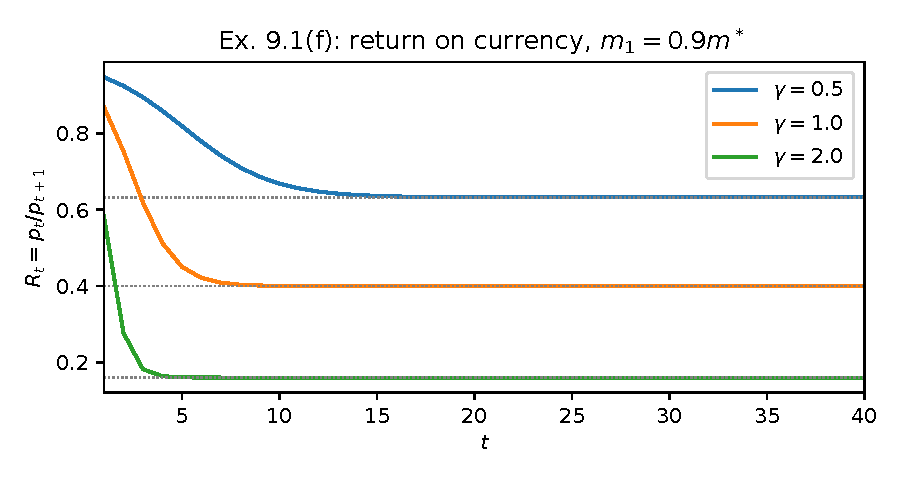
\includegraphics[width=0.72\linewidth]{fig/ls09_9_1_returns.pdf}\\[3pt]
\captionof{figure}{Exercise 9.1(f). $R_t$ along nonstationary equilibria with $m_1=0.9m^*$
($w_1=1$, $w_2=0.4$). Dotted lines: $(w_2/w_1)^\gamma$.}
\end{center}

\begin{tcolorbox}[databox]
Parameters: $w_1=1$, $w_2=.4$, $\gamma\in\{.5,1,2\}$. The closed-form $s(R)$ matches numerical
maximisation to $10^{-6}$. For every $\gamma$, $s(1)=.3=m^*$ is a fixed point. From $m_1=.9m^*$ the
forward map gives a strictly falling $m_t$ and $R_{80}=.632456,\ .400000,\ .160000$, which equals
$(w_2/w_1)^\gamma$.
\end{tcolorbox}
\end{tcolorbox}

%------- 9.2 -------
\begin{tcolorbox}[evenbox,title={Exercise 9.2 \quad Lenders and borrowers in one generation}]
\begin{tcolorbox}[questionbox]
p.~367. Consider an economy with overlapping generations of a constant population of an even number
$N$ of two-period-lived agents. New young agents are born at each date $t\ge1$. Half of the young
agents are endowed with $w_1$ when young and $0$ when old. The other half are endowed with $0$ when
young and $w_2$ when old. Assume $0<w_2<w_1$. Preferences of all young agents are as in problem 1,
with $\gamma=1$. Half of the $N$ initial old are endowed with $w_2$ units of the consumption good and
half are endowed with nothing. Each old person orders consumption streams by $c_1^0$. Each old person
at $t=1$ is endowed with $M$ units of unbacked fiat currency. No other generation is endowed with
fiat currency. The stock of fiat currency is fixed over time.

\textbf{a.} Find the saving function of each of the two types of young person for $t\ge1$.

\textbf{b.} Define an equilibrium without valued fiat currency. Compute all such equilibria.

\textbf{c.} Define an equilibrium with valued fiat currency.

\textbf{d.} Compute all the (nonstochastic) equilibria with valued fiat currency.

\textbf{e.} Argue that there is a unique stationary equilibrium with valued fiat currency.

\textbf{f.} How are the various equilibria with valued fiat currency ranked by the Pareto criterion?
\end{tcolorbox}

\textbf{Solution:} Type 1 has endowment $(w_1,0)$ and type 2 has $(0,w_2)$. $R_t$ is the gross return
on consumption loans (and on currency, when valued). Total currency is $NM$.

\textbf{(a)} By (T1), $s_1(R_t)=w_1/2$ (inelastic) and $s_2(R_t)=-w_2/(2R_t)$ (a borrower).

\textbf{(b)} An \emph{equilibrium without valued currency} is a sequence $\{R_t\}$ and allocations such
that each young person optimises given $R_t$ and the loan market clears,
$\frac N2s_1(R_t)+\frac N2s_2(R_t)=0$, with $1/p_t=0$. The clearing condition reads
$\frac N2\cdot\frac{w_1}2=\frac N2\cdot\frac{w_2}{2R_t}$, so $\boxed{R_t=w_2/w_1}$ for every $t$. The
equilibrium is unique because each date is a separate Fisher loan economy. Both types consume
$(w_1/2,\,w_2/2)$: type 1 gets $c_o=R_tw_1/2=w_2/2$ and type 2 gets $c_y=w_2/(2R_t)=w_1/2$. The
initial old consume their endowments, $w_2$ or $0$.

\textbf{(c)} An \emph{equilibrium with valued fiat currency} is a positive sequence $\{p_t\}$,
$p_t<\infty$, with $R_t=p_t/p_{t+1}$, such that currency and loans bear the same return, each young
person optimises, and the young's net saving equals the old's real balances:
\[
\tfrac N2\big[s_1(R_t)+s_2(R_t)\big]=\frac{NM}{p_t}\quad\Longleftrightarrow\quad \tfrac14\Big(w_1-w_2\frac{p_{t+1}}{p_t}\Big)=\frac M{p_t}.
\]
The initial old consume their goods endowment plus $M/p_1$.

\textbf{(d)} Multiply by $4p_t/w_1$: $p_t=\frac{4M}{w_1}+\frac{w_2}{w_1}p_{t+1}$, the analogue of (9.4.7).
Let $p^*=4M/(w_1-w_2)$ be its fixed point. Then $p_{t+1}-p^*=\frac{w_1}{w_2}(p_t-p^*)$, and
\[
\boxed{p_t=p^*+(p_1-p^*)\Big(\frac{w_1}{w_2}\Big)^{t-1},\qquad p_1\ge p^*.}
\]
If $p_1<p^*$, then $p_t\to-\infty$, which is impossible. Every $p_1\ge p^*$ is an equilibrium. Along
it, $R_t=p_t/p_{t+1}\in[w_2/w_1,1]$ and $R_t\to w_2/w_1$ when $p_1>p^*$. Allocations: type 1 gets
$(w_1/2,R_tw_1/2)$ and type 2 gets $(w_2/(2R_t),w_2/2)$.

\textbf{(e)} Stationarity requires constant real balances $M/p_t$, so $p_t=p$ and $R=1$. From (d),
$p=p^*=4M/(w_1-w_2)$, which is unique. Put differently, $p_1=p^*$ is the only member of the family
with $p_{t+1}=p_t$.

\textbf{(f)} Let $x_t=(p_1-p^*)(w_1/w_2)^{t-1}\ge0$. Then
$R_t=\frac{p^*+x_t}{p^*+x_t w_1/w_2}$, which is strictly decreasing in $x_t$. So a higher $p_1$ lowers
$R_t$ at \emph{every} date. By (T2), lenders (type 1, $s>0$) lose and borrowers (type 2, $s<0$) gain.
The initial old, who hold $M/p_1$, lose. \textbf{The equilibria with valued currency are not Pareto
ranked.} Moving to a lower $p_1$ helps type 1 and the initial old but hurts every type-2 agent. This
contrasts with 9.5, where every young agent is a saver.

\begin{tcolorbox}[databox]
$w_1=1$, $w_2=.5$, $N=2$, $M=1$. \texttt{brentq} on the loan market gives $R=.5=w_2/w_1$. The
closed-form $p_t$ solves the recursion and clears the money market for $p_1\in\{p^*,1.2p^*,2p^*\}$,
$p^*=8$. Comparing $p_1=p^*$ with $1.5p^*$: type-1 utility is higher at every $t$ and type-2 utility
is lower at every $t$.
\end{tcolorbox}
\end{tcolorbox}

%------- 9.3 -------
\begin{tcolorbox}[oddbox,title={Exercise 9.3 \quad A Lucas tree}]
\begin{tcolorbox}[questionbox]
p.~368. Take the economy of exercise 9.1, but make one change. Endow the initial old with a tree
that yields a constant dividend of $d>0$ units of the consumption good for each $t\ge1$.

\textbf{a.} Compute all the equilibria with valued fiat currency.

\textbf{b.} Compute all the equilibria without valued fiat currency.

\textbf{c.} If you want, you can answer both parts of this question in the context of the following
particular numerical example: $w_1=10$, $w_2=5$, $d=.000001$.
\end{tcolorbox}

\textbf{Solution:} \emph{Reading.} As in Example 3 (p.~338), where the feasibility line is
$c_i^i+c_i^{i-1}=y_i^i+y_i^{i-1}+d$, $d$ is the dividend \emph{per young agent} (per capita). Let
$a_t$ be the ex-dividend price of the per-capita tree claim at $t$. Buying it at $t$ pays
$a_{t+1}+d$ at $t+1$. Two conditions hold. Tree arbitrage: $a_tR_t=a_{t+1}+d$. Market clearing:
$s(R_t)=a_t+m_t$.

\textbf{(a) No equilibrium with valued fiat currency exists.} Suppose currency is valued at all $t$.
(If it were worthless at some $t+1$, nobody would buy it at $t$.) Then $R_t=m_{t+1}/m_t$, the tree
must earn the same return, and $0<m_t\le s(R_t)<w_1$. Iterate the arbitrage condition $T$ times:
\[
a_1=\sum_{j=1}^{T}\frac{d}{R_1\cdots R_j}+\frac{a_{T+1}}{R_1\cdots R_T}\ \ge\ \sum_{j=1}^{T}d\,\frac{m_1}{m_{j+1}}\ \ge\ T\,d\,\frac{m_1}{w_1}.
\]
Here $R_1\cdots R_j=m_{j+1}/m_1$ and $a_{T+1}\ge0$. The right side tends to $\infty$ as $T\to\infty$,
but $a_1\le s(R_1)<w_1$. This is a contradiction. Valued money would have to keep a nonvanishing
share of saving, which forces $\prod R_s$ to stay bounded. Then the tree, with its perpetual
dividend, would be worth an unbounded amount.

\textbf{(b)} Without valued currency, $s(R_t)=a_t$ and $a_{t+1}=R_ta_t-d$. A stationary point
satisfies $s(R)(R-1)=d$. Since $d>0$ and $a=s(R)>0$ (a positive-dividend asset has a positive price),
we need $R>1$. For log utility, $a=s(R)=\frac12(w_1-w_2/R)$ gives $R=w_2/(w_1-2a)$, and the map is
\[
a_{t+1}=\varphi(a_t)\equiv\frac{w_2a_t}{w_1-2a_t}-d,\qquad \varphi'(a)=\frac{w_1w_2}{(w_1-2a)^2}.
\]
Fixed points: $(a+d)(w_1-2a)=w_2a$, so $2a^2-(w_1-w_2-2d)a-dw_1=0$. The product of the roots is
$-dw_1/2<0$, so there is one positive root $\bar a$ and one negative root:
\[
\bar a=\frac{(w_1-w_2-2d)+\sqrt{(w_1-w_2-2d)^2+8dw_1}}{4},\qquad \bar R=\frac{\bar a+d}{\bar a}>1,\qquad \bar a=\frac d{\bar R-1}.
\]
At $\bar a$, $\varphi'(\bar a)>1$ ($\bar a$ is near $(w_1-w_2)/2$, so $\varphi'\approx w_1/w_2$). If
$a_1>\bar a$, the path rises until $a_t\ge w_1/2$, which is infeasible. If $a_1<\bar a$, it falls
through $0$ toward the negative root, which is also infeasible. \textbf{The unique equilibrium is
stationary}: $a_t=\bar a$, $R_t=\bar R>1$. It is the book's Example 3 (Figure 9.2.3). For general
$\gamma$ the same graph applies: the candidate with $R<1$ gives the old unbounded wealth.

\textbf{(c)} With $w_1=10$, $w_2=5$, $d=10^{-6}$ and $\gamma=1$: $\bar a=2.5000010$,
$\bar R-1=4.0\times10^{-7}$, $c_y=w_1-\bar a=7.4999990$, $c_o=w_2+\bar a+d\approx7.5$. A
microscopic dividend is enough to eliminate every monetary equilibrium and all the equilibria that
converge to autarky. It selects (almost exactly) the golden-rule allocation $c_y=c_o=7.5$, with the
tree playing the role that fiat money plays in the stationary equilibrium of 9.1(d).

\begin{tcolorbox}[databox]
\texttt{brentq} on $s(R)(R-1)=d$ equals the quadratic root ($\gamma=1$), and gives $R-1=4.0\times10^{-7}$,
$a=2.5000002$ for $\gamma=2$. Paths from $\bar a(1\pm10^{-4})$ leave $(0,w_1/2)$ at $t=14$ (above)
and $t=35$ (below). For (a), the bound $Tdm_1/w_1$ exceeds $w_1$ for large finite $T$.
\end{tcolorbox}
\end{tcolorbox}

%------- 9.4 -------
\begin{tcolorbox}[evenbox,title={Exercise 9.4 \quad Population growth}]
\begin{tcolorbox}[questionbox]
p.~368. Take the economy of exercise 9.1 and make the following two changes. First, assume that
$\gamma=1$. Second, assume that the number of young agents born at $t$ is $N(t)=nN(t-1)$, where
$N(0)>0$ is given and $n\ge1$. Everything else about the economy remains the same.

\textbf{a.} Compute an equilibrium without valued fiat money.

\textbf{b.} Compute a stationary equilibrium with valued fiat money.
\end{tcolorbox}

\textbf{Solution:}

\textbf{(a)} With $1/p_t=0$ and identical young agents, there is no trade: $c_t^t=w_1$,
$c_{t+1}^t=w_2$, $c_1^0=w_2$. The shadow interest factor that makes the young content with zero
saving, $s(R)=0$, is $R=w_2/w_1<1$.

\textbf{(b)} Money-market clearing is $N(t)s(R_t)=M/p_t$. Let $m_t=M/(N(t)p_t)$ be real balances per
young person. Stationarity means $m_t=m$. Then $p_tN(t)$ is constant, so $p_{t+1}/p_t=N(t)/N(t+1)=1/n$
and $\boxed{R_t=n}$ (the high-interest-rate equilibrium). By (T1),
\[
m=s(n)=\tfrac12\Big(w_1-\frac{w_2}n\Big)>0,\qquad p_t=\frac{M}{N(0)n^t\,s(n)}=\frac{2Mn^{1-t}}{N(0)(nw_1-w_2)},
\]
\[
c_y=\tfrac12\Big(w_1+\frac{w_2}n\Big),\qquad c_o=w_2+nm=\tfrac12(nw_1+w_2),\qquad c_1^0=w_2+\frac{M}{N(0)p_1}=w_2+nm.
\]
$s(n)>0$ because $nw_1\ge w_1>w_2$. Feasibility per young person, $c_y+c_o/n=w_1+w_2/n$, holds. The
price level falls at rate $n$, so currency pays the population growth rate.

\begin{tcolorbox}[databox]
$w_1=1$, $w_2=.4$, $n=1.1$: $s(n)=0.318182$, $(c_y,c_o)=(0.681818,\,0.75)$. We verify $R_t=n$ and
market clearing at every date, the feasibility identity, and that the closed-form $s(n)$ equals the
numerical optimum.
\end{tcolorbox}
\end{tcolorbox}

%------- 9.5 -------
\begin{tcolorbox}[oddbox,title={Exercise 9.5 \quad All monetary equilibria with growth}]
\begin{tcolorbox}[questionbox]
p.~368. Consider an economy consisting of overlapping generations of two-period-lived consumers. At
each date $t\ge1$ there are born $N(t)$ identical young people each of whom is endowed with $w_1>0$
units of a single consumption good when young and $w_2>0$ units of the consumption good when old.
Assume that $w_2<w_1$. The consumption good is not storable. The population of young people is
described by $N(t)=nN(t-1)$, where $n>0$. Young people born at $t$ rank utility streams according to
$\ln(c_t^t)+\ln(c_{t+1}^t)$ where $c_t^i$ is the consumption of the time $t$ good of an agent born in
$i$. In addition, there are $N(0)$ old people at time 1, each of whom is endowed with $w_2$ units of
the time 1 consumption good. The old at $t=1$ are also endowed with one unit of unbacked pieces of
infinitely durable but intrinsically worthless pieces of paper called fiat money.

\textbf{a.} Define an equilibrium without valued fiat currency. Compute such an equilibrium.

\textbf{b.} Define an equilibrium with valued fiat currency.

\textbf{c.} Compute all equilibria with valued fiat currency.

\textbf{d.} Find the limiting rates of return on currency as $t\to+\infty$ in each of the equilibria
that you found in part c. Compare them with the one-period interest rate in the equilibrium in part a.

\textbf{e.} Are the equilibria in part c ranked according to the Pareto criterion?
\end{tcolorbox}

\textbf{Solution:} \emph{Reading.} ``One unit'' is per initial old person, so the currency stock is
$N(0)$.

\textbf{(a)} An \emph{equilibrium without valued currency} is $1/p_t=0$ with each young agent
optimising given the loan rate $R_t$, and zero aggregate saving, $N(t)s(R_t)=0$. Since the agents are
identical, $s(R_t)=0$, so $R_t=w_2/w_1$ (autarky: $c_t^t=w_1$, $c_{t+1}^t=w_2$, $c_1^0=w_2$).

\textbf{(b)} An \emph{equilibrium with valued currency} is a positive sequence $\{p_t\}$, $p_t<\infty$,
such that, with $R_t=p_t/p_{t+1}$, each young agent saves $s(R_t)=\frac12(w_1-w_2/R_t)$ and
$N(t)s(R_t)=N(0)/p_t$. Consumption is $c_t^t=w_1-s(R_t)$, $c_{t+1}^t=w_2+R_ts(R_t)$, and
$c_1^0=w_2+1/p_1$.

\textbf{(c)} Multiply the clearing condition by $2p_t/N(t)$, using $N(0)/N(t)=n^{-t}$:
$2n^{-t}=w_1p_t-w_2p_{t+1}$, that is
\[
p_{t+1}=\frac{w_1}{w_2}p_t-\frac{2}{w_2}n^{-t}.
\]
\emph{Particular solution.} Try $p_t=Kn^{-t}$: $Kn^{-t-1}=\frac{w_1}{w_2}Kn^{-t}-\frac2{w_2}n^{-t}$, so
$K\big(\frac{w_1}{w_2}-\frac1n\big)=\frac2{w_2}$ and $K=\frac{2n}{nw_1-w_2}$. \emph{General
solution:}
\[
\boxed{p_t=\frac{2n}{nw_1-w_2}\,n^{-t}+c\Big(\frac{w_1}{w_2}\Big)^t .}
\]
\emph{Case $nw_1>w_2$} ($n>w_2/w_1=\theta_{\rm aut}$). Here $K>0$ and $w_1/w_2>1/n$. If $c<0$, the
second term dominates and $p_t<0$ eventually. So the equilibria are exactly $c\ge0$ (a continuum),
with $c=0$ the stationary one: real balances per young $s(n)$ constant.
\emph{Case $nw_1\le w_2$.} If $nw_1<w_2$, then $K<0$ and $1/n>w_1/w_2$, so the first term dominates
and $p_t<0$ eventually for every $c$. If $nw_1=w_2$, write $p_t=q_tn^{-t}$; then
$q_{t+1}=q_t-2n/w_2\to-\infty$. Either way there is \textbf{no} monetary equilibrium. This is the
proposition of section 9.7 with $z=1$: one exists iff $\theta_{\rm aut}<n$.

\textbf{(d)} For $c=0$, $R_t=n$ for all $t$. For $c>0$, $p_t\sim c(w_1/w_2)^t$, so
$R_t=p_t/p_{t+1}\to w_2/w_1$. That is the one-period interest factor of the nonmonetary equilibrium in
(a). The nonstationary equilibria are asymptotically autarkic.

\textbf{(e)} \textbf{Yes, they are completely ranked.} Write $a_t=Kn^{-t}>0$ and $b_t=c(w_1/w_2)^t\ge0$.
Then
\[
R_t=\frac{a_t+b_t}{a_t/n+b_t\,w_1/w_2},
\]
a weighted average (in the sense of a ratio of sums) of $n$ and $w_2/w_1$. Its weight shifts
toward $w_2/w_1<n$ as $b_t/a_t$ rises, and $b_t/a_t$ is increasing in $c$. So a higher $c$ lowers
$R_t$ at every $t$. Every young agent is a saver ($s(R_t)=m_t>0$), so by (T2) $v(R_t)$ falls: every
generation $t\ge1$ is worse off. The initial old consume $w_2+1/p_1$, which falls with $c$. The
stationary equilibrium ($c=0$) Pareto dominates every other, and a lower $c$ dominates a higher $c$.
Since $n>\theta_{\rm aut}$ and $z=1$, the stationary one is Pareto optimal (section 9.7). The others
converge to the nonoptimal autarky.

\begin{tcolorbox}[databox]
$w_1=1$, $w_2=.5$, $n=.9$ ($K=4.5$). For $c\in\{0,10^{-6},10^{-3},1\}$ the closed form solves the
recursion and clears the money market. $R_{200}$ equals $n$ ($c=0$) or $w_2/w_1$ ($c>0$). Utilities of
all 199 generations and $1/p_1$ decrease with $c$. With $n=.4<w_2/w_1$, every $c\ge0$ gives $p_t<0$
within 60 periods.
\end{tcolorbox}
\end{tcolorbox}

%----------------------------------------------------------------------
\subsection{Several Currencies, Credit, and Inside Money}
%----------------------------------------------------------------------

%------- 9.6 -------
\begin{tcolorbox}[evenbox,title={Exercise 9.6 \quad Exchange rate determinacy}]
\begin{tcolorbox}[questionbox]
pp.~369--370. The world consists of two economies, named $i=1,2$, which except for their
governments' policies are ``copies'' of one another. At each date $t\ge1$, there is a single
consumption good, which is storable, but only for rich people. Each economy consists of overlapping
generations of two-period-lived agents. For each $t\ge1$, in economy $i$, $N$ poor people and $N$
rich people are born. Let $c_t^h(s),y_t^h(s)$ be the time $s$ (consumption, endowment) of a type $h$
agent born at $t$. Poor agents are endowed with $[y_t^h(t),y_t^h(t+1)]=(\alpha,0)$; rich agents are
endowed with $[y_t^h(t),y_t^h(t+1)]=(\beta,0)$, where $\beta\gg\alpha$. In each country, there are
$2N$ initial old who are endowed in the aggregate with $H_i(0)$ units of an unbacked currency and
with $2N\epsilon$ units of the time 1 consumption good. For the rich people, storing $k$ units of the
time $t$ consumption good produces $Rk$ units of the time $t+1$ consumption good, where $R>1$ is a
fixed gross rate of return on storage. Rich people can earn the rate of return $R$ either by storing
goods or by lending to either government by means of indexed bonds. We assume that poor people are
prevented from storing capital or holding indexed government debt by the sort of denomination and
intermediation restrictions described by Sargent and Wallace (1982).

For each $t\ge1$, all young agents order consumption streams according to
$\ln c_t^h(t)+\ln c_t^h(t+1)$.

For $t\ge1$, the government of country $i$ finances a stream of purchases (to be thrown into the
ocean) of $G_i(t)$ subject to the following budget constraint:
\[
(1)\qquad G_i(t)+RB_i(t-1)=B_i(t)+\frac{H_i(t)-H_i(t-1)}{p_i(t)}+T_i(t),
\]
where $B_i(0)=0$; $p_i(t)$ is the price level in country $i$; $T_i(t)$ are lump-sum taxes levied by
the government on the \emph{rich} young people at time $t$; $H_i(t)$ is the stock of $i$'s fiat
currency at the end of period $t$; $B_i(t)$ is the stock of indexed government interest-bearing debt
(held by the rich of either country). The government does not explicitly tax poor people, but might
tax through an inflation tax. Each government levies a lump-sum tax of $T_i(t)/N$ on each young rich
citizen of its own country.

Poor people in both countries are free to hold whichever currency they prefer. Rich people can hold
debt of either government and can also store; storage and both government debts bear a constant
gross rate of return $R$.

\textbf{a.} Define an \emph{equilibrium} with valued fiat currencies (in both countries).

\textbf{b.} In a nonstochastic equilibrium, verify the following proposition: if an equilibrium
exists in which both fiat currencies are valued, the exchange rate between the two currencies must
be constant over time.

\textbf{c.} Suppose that government policy in each country is characterized by specified
(exogenous) levels $G_i(t)=G_i$, $T_i(t)=T_i$, $B_i(t)=0$, $\forall t\ge1$. (The remaining elements
of government policy adjust to satisfy the government budget constraints.) Assume that the exogenous
components of policy have been set so that an equilibrium with two valued fiat currencies exists.
Under this description of policy, show that the equilibrium exchange rate is indeterminate.

\textbf{d.} Suppose that government policy in each country is described as follows:
$G_i(t)=G_i$, $T_i(t)=T_i$, $H_i(t+1)=H_i(1)$, $B_i(t)=B_i(1)$ $\forall t\ge1$. Show that if there
exists an equilibrium with two valued fiat currencies, the exchange rate is determinate.

\textbf{e.} Suppose that government policy in country 1 is specified in terms of exogenous levels of
$s_1=[H_1(t)-H_1(t-1)]/p_1(t)$ $\forall t\ge2$, and $G_1(t)=G_1$ $\forall t\ge1$. For country 2,
government policy consists of exogenous levels of $B_2(t)=B_2(1)$, $G_2(t)=G_2$ $\forall t\ge1$. Show
that if there exists an equilibrium with two valued fiat currencies, then the exchange rate is
determinate.
\end{tcolorbox}

\textbf{Solution:} Write $R_{it}=p_i(t)/p_i(t+1)$ for the gross return on currency $i$ (distinct from
the storage return $R$), $h_i(t)=H_i(t)/p_i(t)$ for its real stock, and $e(t)=p_1(t)/p_2(t)$ for the
exchange rate. By (T1) with endowment $(y,0)$, each young person saves half the after-tax endowment,
whatever the return. The $2N$ poor of the world therefore demand $N\alpha$ of real balances in total.
The rich save $(\beta-T_i/N)/2$ each, in storage or bonds at $R$.

\textbf{(a)} An \emph{equilibrium with two valued currencies} consists of positive finite sequences
$\{p_1(t),p_2(t)\}$, stocks $\{H_i(t),B_i(t)\}$, storage, and allocations, for given policy, such that
five conditions hold.
(i) The poor maximise: $c^{\rm poor}(t)=\alpha/2$, and they hold only currencies with the highest
return, $\max_iR_{it}$.
(ii) The rich maximise: they save $(\beta-T_i(t)/N)/2$ in storage and bonds, and hold currency only
if its return is at least $R$.
(iii) The world currency market clears, $h_1(t)+h_2(t)=N\alpha$, with $h_i(t)>0$ for both $i$.
(iv) The rich's saving equals storage plus $B_1(t)+B_2(t)$.
(v) Both budget constraints (1) hold, and goods markets clear.

\textbf{(b)} Both currencies are held by the poor at every $t$. If $R_{1t}>R_{2t}$, no one would hold
currency 2 at $t$, so $h_2(t)=0$, a contradiction. Hence $R_{1t}=R_{2t}$, that is
$\frac{p_1(t)}{p_1(t+1)}=\frac{p_2(t)}{p_2(t+1)}$. Rearranged, $\frac{p_1(t+1)}{p_2(t+1)}=\frac{p_1(t)}{p_2(t)}$,
so $e(t+1)=e(t)=e$.

\textbf{(c)} With $B_i=0$, (1) gives $[H_i(t)-H_i(t-1)]/p_i(t)=G_i-T_i\equiv d_i$ for every $t\ge1$.
Let $R_m$ be the common currency return. Then
$h_i(t)=\frac{H_i(t-1)}{p_i(t-1)}\frac{p_i(t-1)}{p_i(t)}+d_i=R_mh_i(t-1)+d_i$ for $t\ge2$. Summing over
$i$ and using (iii): $N\alpha=R_mN\alpha+d_1+d_2$, so $R_m=1-(d_1+d_2)/(N\alpha)$, a constant. At
$t=1$, with $p_2(1)=p_1(1)/e$, the two budgets add to
\[
\frac{H_1(0)+e\,H_2(0)}{p_1(1)}+d_1+d_2=N\alpha .
\]
This is \emph{one} equation in two unknowns $(p_1(1),e)$. Pick any $e>0$. Then
$p_1(1)=\frac{H_1(0)+eH_2(0)}{N\alpha-d_1-d_2}$, $p_i(t)=p_i(1)R_m^{1-t}$, and
$h_i(t)=R_m^{t-1}[h_i(1)-\bar h_i]+\bar h_i>0$ with $\bar h_i=d_i/(1-R_m)$. Every condition of (a)
holds: the poor consume $(\alpha/2,R_m\alpha/2)$, the rich and the governments are unaffected, and
$R_m<R$. So \textbf{every $e\in(0,\infty)$ is an equilibrium exchange rate} (Kareken--Wallace). The
real allocation is the same for all $e$. Only the split of world real balances between the two
currencies and between the two countries' initial old depends on $e$. \emph{Remark.} Only one $e$
keeps each currency's real stock constant, $e=\frac{H_1(0)d_2}{H_2(0)d_1}$ (needs $d_1,d_2>0$). This
is the book's section 27.3.11 selection; the definition in (a) does not impose it.

\textbf{(d)} Now the nominal stocks $H_i(t)=H_i(1)$ and bonds $B_i(1)$ are policy. For $t\ge2$, (1)
reads $G_i+RB_i(1)=B_i(1)+0+T_i$, a restriction on policy: $(R-1)B_i(1)=T_i-G_i$. With $e$ constant
and both stocks constant, (iii) gives $\frac{H_1(1)+eH_2(1)}{p_1(t)}=N\alpha$, so $p_1(t)$ and
$p_2(t)$ are constant for $t\ge1$ and $R_m=1$. The $t=1$ budget, $G_i=B_i(1)+[H_i(1)-H_i(0)]/p_i(1)+T_i$,
now \emph{pins each price level separately}:
\begin{gather*}
S_i\equiv G_i-T_i-B_i(1)=\frac{R}{R-1}(G_i-T_i),\qquad p_i(1)=\frac{H_i(1)-H_i(0)}{S_i},\\
\boxed{e=\frac{[H_1(1)-H_1(0)]\,S_2}{[H_2(1)-H_2(0)]\,S_1}.}
\end{gather*}
Existence requires the policies to satisfy $H_1(1)/p_1+H_2(1)/p_2=N\alpha$; that is the ``if there
exists'' clause. If one country has $S_i=0$ (so $H_i(1)=H_i(0)$), its price level is still
determined, by (iii) given the other's. Only when both have $S_i=0$ do we return to indeterminacy.
The difference from (c) is that the governments now fix \emph{nominal} quantities, which anchor each
currency's value through its own budget constraint.

\textbf{(e)} \emph{Reading.} The statement leaves some instruments unnamed. We keep $T_i(t)=T_i$ from
(c)--(d) in both countries, and let each country's remaining element adjust. For country 1 that is
$B_1$, subject to boundedness: the rich's saving is bounded. For country 2 it is currency, as a
one-time nominal issue $H_2(1)$ that is then held fixed (as in (d)). \emph{Country 2.} For $t\ge2$,
(1) requires $T_2=G_2+(R-1)B_2(1)$. At $t=1$, $p_2(1)=[H_2(1)-H_2(0)]/(G_2-T_2-B_2(1))$ is pinned,
exactly as in (d). \emph{Country 1.} For $t\ge2$, $B_1(t)=RB_1(t-1)+G_1-T_1-s_1$. Its solution is
$B_1(t)=\bar b+R^{t-1}(B_1(1)-\bar b)$ with $\bar b=(T_1+s_1-G_1)/(R-1)$. Since $R>1$, boundedness
forces $B_1(1)=\bar b$, and then the $t=1$ seigniorage is pinned too:
$\sigma_1\equiv[H_1(1)-H_1(0)]/p_1(1)=G_1-T_1-\bar b$. \emph{World money market.} For $t\ge2$,
$N\alpha=R_mN\alpha+s_1$, so $R_m=1-s_1/(N\alpha)$. At $t=1$,
\[
\frac{H_1(0)}{p_1(1)}+\sigma_1+\frac{H_2(1)}{p_2(1)}=N\alpha
\quad\Longrightarrow\quad p_1(1)=\frac{H_1(0)}{N\alpha-\sigma_1-H_2(1)/p_2(1)} ,
\]
which is unique. Hence $e=p_1(1)/p_2(1)$ is \textbf{determinate}, and constant by (b). Country 2's
nominal anchor fixes $p_2$, and world money demand then fixes $p_1$. \emph{Caveat.} If country 2
instead financed $G_2+(R-1)B_2$ by money creation every period with $T_2$ fixed, both governments
would be setting real seigniorage. The $t=1$ condition would again be one equation in $(p_1(1),e)$,
as in (c), and $e$ would be indeterminate. Determinacy needs at least one nominal anchor.

\begin{tcolorbox}[databox]
(c) with $N\alpha=1$, $H_1(0)=2$, $H_2(0)=3$, $d_1=.05$, $d_2=.10$: for $e\in\{0.2,1,5\}$ the world
market clears at every date, $R_m=.85$ for all $e$, and both real stocks stay positive and converge to
$d_i/(1-R_m)$. $e=4/3$ gives the constant split. (d) with $H_i(1)=1.1H_i(0)$, $S_1=.04$, $S_2=.06$:
$p_1=p_2=5$, $e=1$, and existence requires $N\alpha=1.1$.
\end{tcolorbox}
\end{tcolorbox}

%------- 9.7 -------
\begin{tcolorbox}[oddbox,title={Exercise 9.7 \quad Credit controls}]
\begin{tcolorbox}[questionbox]
pp.~370--371. Consider the following overlapping generations model. At each date $t\ge1$ there
appear $N$ two-period-lived young people, said to be of generation $t$, who live and consume during
periods $t$ and $(t+1)$. At time $t=1$ there exist $N$ old people who are endowed with $H(0)$ units of
paper ``dollars,'' which they offer to supply inelastically to the young of generation 1 in exchange
for goods. Let $p(t)$ be the price of the one good in the model, measured in dollars per time $t$
good. For each $t\ge1$, $N/2$ members of generation $t$ are endowed with $y>0$ units of the good at
$t$ and $0$ units at $(t+1)$, whereas the remaining $N/2$ members of generation $t$ are endowed with
$0$ units of the good at $t$ and $y>0$ units when they are old. All members of all generations have
the same utility function:
\[
u[c_t^h(t),c_t^h(t+1)]=\ln c_t^h(t)+\ln c_t^h(t+1),
\]
where $c_t^h(s)$ is the consumption of agent $h$ of generation $t$ in period $s$. The old at $t=1$
simply maximize $c_0^h(1)$. The consumption good is nonstorable. The currency supply is constant
through time, so $H(t)=H(0)$, $t\ge1$.

\textbf{a.} Define a competitive equilibrium without valued currency for this model. Who trades what
with whom?

\textbf{b.} In the equilibrium without valued fiat currency, compute competitive equilibrium values
of the gross return on consumption loans, the consumption allocation of the old at $t=1$, and that of
the ``borrowers'' and ``lenders'' for $t\ge1$.

\textbf{c.} Define a competitive equilibrium with valued currency. Who trades what with whom?

\textbf{d.} Prove that for this economy there does not exist a competitive equilibrium with valued
currency.

\textbf{e.} Now suppose that the government imposes the restriction that
$l_t^h(t)[1+r(t)]\ge-y/4$, where $l_t^h(t)[1+r(t)]$ represents claims on $(t+1)$-period consumption
purchased (if positive) or sold (if negative) by household $h$ of generation $t$. This is a
restriction on the amount of borrowing. For an equilibrium without valued currency, compute the
consumption allocation and the gross rate of return on consumption loans.

\textbf{f.} In the setup of part e, show that there exists an equilibrium with valued currency in
which the price level obeys the quantity theory equation $p(t)=qH(0)/N$. Find a formula for the
undetermined coefficient $q$. Compute the consumption allocation and the equilibrium rate of return
on consumption loans.

\textbf{g.} Are lenders better off in economy b or economy f? What about borrowers? What about the
old of period 1 (generation 0)?
\end{tcolorbox}

\textbf{Solution:} ``Lenders'' have $(y,0)$ and ``borrowers'' have $(0,y)$. Let $l_t^h(t)$ be loans
made (negative if borrowed). By (T1), a lender saves $y/2$ and an unconstrained borrower sets
$l=-y/(2[1+r(t)])$, promising $y/2$ whatever the rate.

\textbf{(a)} A \emph{competitive equilibrium without valued currency} is $1/p(t)=0$ and a sequence
$\{r(t)\}$ with allocations such that each young agent maximises utility given $1+r(t)$, and the loan
market clears, $\frac N2l^{\rm lend}(t)+\frac N2l^{\rm borr}(t)=0$. Young lenders trade time-$t$
goods with young borrowers of the \emph{same} generation, for claims on time-$(t+1)$ goods. There is
no trade across generations. The initial old have no goods and worthless paper.

\textbf{(b)} Clearing: $\frac N2\cdot\frac y2=\frac N2\cdot\frac y{2[1+r(t)]}$, so
$\boxed{1+r(t)=1}$. Lenders consume $(y/2,y/2)$. Borrowers consume $c(t)=y/2$ and
$c(t+1)=y-y/2=y/2$. The initial old consume $c_0^h(1)=0$.

\textbf{(c)} A \emph{competitive equilibrium with valued currency} is a positive finite sequence
$\{p(t)\}$ with $1+r(t)=p(t)/p(t+1)$ (currency and loans are perfect substitutes) such that agents
optimise and $\frac N2l^{\rm lend}(t)+\frac N2l^{\rm borr}(t)=H(0)/p(t)$. The old sell dollars to the
young (both generations trade), and lenders also lend to borrowers.

\textbf{(d)} Let $m_t=H(0)/p(t)$. Clearing gives $m_t=\frac{Ny}4\big[1-\frac1{1+r(t)}\big]$, so
$m_t>0$ requires $1+r(t)>1$. With $1+r(t)=m_{t+1}/m_t$, let $x_t=4m_t/(Ny)\in(0,1)$. Then
$1+r(t)=1/(1-x_t)$ and $x_{t+1}=x_t/(1-x_t)$, that is
\[
\frac1{x_{t+1}}=\frac1{x_t}-1\quad\Longrightarrow\quad \frac1{x_t}=\frac1{x_1}-(t-1),
\]
which is $\le1$ for $t\ge1/x_1$. So $x_t\ge1$ (or negative), which contradicts $x_t<1$. \textbf{No
equilibrium with valued currency exists.} This matches section 9.7. The nonmonetary equilibrium has
$1+r=1=n$, so it is already optimal ($\theta_{\rm aut}=n$). Money would need a return above $1$
forever, which requires ever-growing real balances.

\textbf{(e)} The borrower wants to promise $y/2$ but may promise only $y/4$. The constraint binds at
any rate: borrowing is $y/(4[1+r])$. Clearing: $\frac N2\cdot\frac y2=\frac N2\cdot\frac y{4[1+r]}$, so
$\boxed{1+r(t)=\tfrac12}$. Lenders consume $(y/2,\,y/4)$. Borrowers consume
$\big(\frac y{4\cdot\frac12},\,y-\frac y4\big)=(y/2,\,3y/4)$. The initial old consume $0$.

\textbf{(f)} Try $p(t)=p$ constant, so $1+r(t)=1$. Lenders save $y/2$. Borrowers are still
constrained at $1+r=1$ (they want $y/2>y/4$), so they borrow $y/4$. Net saving of the young equals
real balances:
\[
\tfrac N2\Big(\frac y2-\frac y4\Big)=\frac{Ny}8=\frac{H(0)}p
\quad\Longrightarrow\quad p=\frac{8H(0)}{Ny}=q\frac{H(0)}N,\qquad \boxed{q=\frac8y}.
\]
The allocation is: lenders $(y/2,y/2)$, borrowers $(y/4,3y/4)$, each initial old $H(0)/(Np)=y/8$. The
return on consumption loans is $1+r=1$. Check at $t\ge2$: $\frac N2(\frac y2+\frac y4)+\frac N2(\frac
y2+\frac{3y}4)=Ny$. At $t=1$: $\frac N2\cdot\frac{3y}4+N\frac y8=\frac N2y$. Both equal the endowment.
\checkmark

\textbf{(g)} Lenders consume $(y/2,y/2)$ in both b and f, so they are \emph{indifferent}. Borrowers get
$2\ln y-2\ln2$ in b and $2\ln y+\ln\frac3{16}$ in f. Since $\frac3{16}<\frac14$, they are
\emph{worse off} in f. The initial old get $0$ in b and $y/8$ in f, so they are \emph{better off}.
The credit control and valued money together transfer resources from borrowers to generation 0.

\begin{tcolorbox}[databox]
$y=1$, $N=2$, $H(0)=1$. \texttt{brentq} gives $1+r=1$ (b) and $\tfrac12$ (e). The iteration
$x\mapsto x/(1-x)$ leaves $(0,1)$ from $x_1\in\{10^{-3},.1,.5\}$. We check $q=8$, feasibility at $t=1$
and $t\ge2$, and the three welfare comparisons.
\end{tcolorbox}
\end{tcolorbox}

%------- 9.8 -------
\begin{tcolorbox}[evenbox,title={Exercise 9.8 \quad Inside money and real bills}]
\begin{tcolorbox}[questionbox]
pp.~371--373. Consider the following overlapping generations model of two-period-lived people. At
each date $t\ge1$ there are born $N_1$ individuals of type 1 who are endowed with $y>0$ units of the
consumption good when they are young and zero units when they are old; there are also born $N_2$
individuals of type 2 who are endowed with zero units of the consumption good when they are young
and $Y>0$ units when they are old. The consumption good is nonstorable. At time $t=1$, there are $N$
old people, all of the same type, each endowed with zero units of the consumption good and $H_0/N$
units of unbacked paper called ``fiat currency.'' The populations of type 1 and 2 individuals, $N_1$
and $N_2$, remain constant for all $t\ge1$. The young of each generation are identical in preferences
and maximize the utility function $\ln c_t^h(t)+\ln c_t^h(t+1)$ where $c_t^h(s)$ is consumption in the
$s$th period of a member $h$ of generation $t$.

\textbf{a.} Consider the equilibrium without valued currency (that is, the equilibrium in which there
is no trade between generations). Let $[1+r(t)]$ be the gross rate of return on consumption loans.
Find a formula for $[1+r(t)]$ as a function of $N_1,N_2,y$, and $Y$.

\textbf{b.} Suppose that $N_1,N_2,y$, and $Y$ are such that $[1+r(t)]>1$ in the equilibrium without
valued currency. Then prove that there can exist no quantity-theory-style equilibrium where fiat
currency is valued and where the price level $p(t)$ obeys the quantity theory equation $p(t)=q\cdot
H_0$, where $q$ is a positive constant and $p(t)$ is measured in units of currency per unit good.

\textbf{c.} Suppose that $N_1,N_2,y$, and $Y$ are such that in the nonvalued-currency equilibrium
$1+r(t)<1$. Prove that there exists an equilibrium in which fiat currency is valued and that there
obtains the quantity theory equation $p(t)=q\cdot H_0$, where $q$ is a constant. Construct an argument
to show that the equilibrium with valued currency is not Pareto superior to the nonvalued-currency
equilibrium.

\textbf{d.} Suppose that $N_1,N_2,y$, and $Y$ are such that, in the preceding nonvalued-currency
economy, $[1+r(t)]<1$, there exists an equilibrium in which fiat currency is valued. Let $\bar p$ be
the stationary equilibrium price level in that economy. Now consider an alternative economy,
identical with the preceding one in all respects except for the following feature: a government each
period purchases a constant amount $L_g$ of consumption loans and pays for them by issuing debt on
itself, called ``inside money'' $M_I$, in the amount $M_I(t)=L_g\cdot p(t)$. The government never
retires the inside money, using the proceeds of the loans to finance new purchases of consumption
loans in subsequent periods. The quantity of outside money, or currency, remains $H_0$, whereas the
``total high-power money'' is now $H_0+M_I(t)$.

(i) Show that in this economy there exists a valued-currency equilibrium in which the price level is
constant over time at $p(t)=\bar p$, or equivalently, with $\bar p=qH_0$ where $q$ is defined in
part c.

(ii) Explain why government purchases of private debt are not inflationary in this economy.

(iii) In many models, once-and-for-all government open-market operations in private debt normally
affect real variables and/or price level. What accounts for the difference between those models and
the one in this exercise?
\end{tcolorbox}

\textbf{Solution:} \emph{Reading.} $N$ (initial old) is not otherwise defined; its value plays no
role. By (T1), type 1 saves $y/2$ and type 2 borrows $Y/(2[1+r])$. Aggregate saving is
$S(R)=\frac12\big(N_1y-N_2\frac YR\big)$, $R=1+r$.

\textbf{(a)} $S(R)=0$ gives $\boxed{1+r(t)=\dfrac{N_2Y}{N_1y}}$.

\textbf{(b)} Suppose $p(t)=qH_0$ for all $t$. Then currency, and hence loans, return
$p(t)/p(t+1)=1$. Clearing requires $S(1)=H_0/p=1/q>0$. But $S(1)=\frac12(N_1y-N_2Y)$, and
$1+r=N_2Y/(N_1y)>1$ means $N_1y<N_2Y$, so $S(1)<0$. This is a contradiction, so no such equilibrium
exists.

\textbf{(c)} Now $N_1y>N_2Y$, so $S(1)>0$. Set $p(t)=qH_0$ with
$\boxed{q=\dfrac{2}{N_1y-N_2Y}}$. Then $R=1$ and $S(1)=H_0/p(t)$ at every date, which is an
equilibrium. Consumption at $R=1$: type 1 gets $(y/2,y/2)$, type 2 gets $(Y/2,Y/2)$, and the initial
old share $1/q$. \emph{Not Pareto superior:} by (T2), a type-2 agent's utility
$\ln\frac Y{2R}+\ln\frac Y2$ is strictly decreasing in $R$. The monetary equilibrium raises $R$ from
$N_2Y/(N_1y)<1$ to $1$, so every type-2 agent of every generation is strictly worse off. Type 1 and
the initial old gain. The two equilibria are Pareto non-comparable.

\textbf{(d)(i)} The government lends $L_g$ each period and finances it with $M_I(t)=L_gp(t)$. Lenders'
saving is held as outside money, inside money, and private loans. Borrowers borrow from private
lenders and from the government. So the loan market condition becomes (the analogue of (9.8.3))
\[
\tfrac12N_1y=\frac{H_0+M_I(t)}{p(t)}+\Big(\tfrac12N_2\frac YR-L_g\Big)
\quad\Longleftrightarrow\quad S(R_t)=\frac{H_0}{p(t)}+\underbrace{\frac{M_I(t)}{p(t)}-L_g}_{=0}.
\]
At $p(t)=\bar p=qH_0$, $R=1$ and $S(1)=H_0/\bar p$ holds by (c). The government's budget: it collects
$RL_g=L_g$ at $t+1$ and relends it, and $M_I=L_g\bar p$ stays constant, so no retirement is needed.
Hence $p(t)=\bar p$ is an equilibrium, and the allocation is the same as in (c).

\textbf{(ii)} Each dollar of inside money is backed one-for-one by a real loan of equal value and
equal return. The public holds $L_g$ more of real balances and $L_g$ less of private loans. Net
saving available to absorb \emph{outside} money, $S(R)$, is unchanged, and so is $p$. This is the
irrelevance of open-market operations (9.8.4)--(9.8.6), Adam Smith's real bills doctrine.

\textbf{(iii)} Here currency and private loans are \emph{perfect substitutes}: same return, no legal
restrictions, no reserve requirements, no denomination barriers. The government's asset swap is then
undone one-for-one by private portfolios (a Modigliani--Miller result for the government's balance
sheet, Wallace 1981). Open-market operations matter in models where (1) legal restrictions separate
the money and credit markets (Sargent--Wallace 1982), so that money pays less than loans; or (2) the
assets bought are not perfect substitutes for money (liquidity, risk, cash-in-advance constraints);
or (3) the operation changes the path of taxes or the backing of money, for instance when the
government buys its own interest-bearing debt that must be serviced by future taxes.

\begin{tcolorbox}[databox]
$N_1=3$, $N_2=2$, $y=Y=1$, $H_0=1$, $L_g=.1$: $1+r=2/3$ by \texttt{brentq} and by formula, $q=2$.
Type-2 utility is lower at $R=1$. With inside money, lenders' saving
$=(H_0+M_I)/\bar p+$ private loans exactly at $\bar p$.
\end{tcolorbox}
\end{tcolorbox}

%----------------------------------------------------------------------
\subsection{Transfers, Seigniorage, and Deficit Finance}
%----------------------------------------------------------------------

%------- 9.9 -------
\begin{tcolorbox}[oddbox,title={Exercise 9.9 \quad Social security and the price level}]
\begin{tcolorbox}[questionbox]
p.~373. Consider an economy (``economy I'') that consists of overlapping generations of
two-period-lived people. At each date $t\ge1$ there is born a constant number $N$ of young people,
who desire to consume both when they are young, at $t$, and when they are old, at $(t+1)$. Each young
person has the utility function $\ln c_t(t)+\ln c_t(t+1)$, where $c_s(t)$ is time $t$ consumption of
an agent born at $s$. For all dates $t\ge1$, young people are endowed with $y>0$ units of a single
nonstorable consumption good when they are young and zero units when they are old. In addition, at
time $t=1$ there are $N$ old people endowed in the aggregate with $H$ units of unbacked fiat currency.
Let $p(t)$ be the nominal price level at $t$, denominated in dollars per time $t$ good.

\textbf{a.} Define and compute an equilibrium with valued fiat currency for this economy. Argue that
it exists and is unique. Now consider a second economy (``economy II'') that is identical to economy
I except that economy II possesses a social security system. In particular, at each date $t\ge1$, the
government taxes $\tau>0$ units of the time $t$ consumption good away from each young person and at
the same time gives $\tau$ units of the time $t$ consumption good to each old person then alive.

\textbf{b.} Does economy II possess an equilibrium with valued fiat currency? Describe the
restrictions on the parameter $\tau$, if any, that are needed to ensure the existence of such an
equilibrium.

\textbf{c.} If an equilibrium with valued fiat currency exists, is it unique?

\textbf{d.} Consider the \emph{stationary} equilibrium with valued fiat currency. Is it unique?
Describe how the value of currency or price level would vary across economies with differences in
the size of the social security system, as measured by $\tau$.
\end{tcolorbox}

\textbf{Solution:}

\textbf{(a)} An \emph{equilibrium with valued currency} is a positive finite $\{p(t)\}$ such that,
with $R_t=p(t)/p(t+1)$, each young agent saves $s(R_t)$ and $Ns(R_t)=H/p(t)$. With endowment $(y,0)$,
(T1) gives $s=y/2$ \emph{for every} $R_t$. So $H/p(t)=Ny/2$ and
\[
\boxed{p(t)=\frac{2H}{Ny}\ \ \forall t,\qquad c_t(t)=c_t(t+1)=\frac y2,\qquad c_0(1)=\frac y2.}
\]
It exists because $y>0$. It is unique because saving is interest-inelastic: the clearing condition
pins $p(t)$ date by date, with no forward-looking term.

\textbf{(b)} In economy II the young's net endowment is $(y-\tau,\tau)$, so
$s(R_t)=\frac12\big(y-\tau-\frac\tau{R_t}\big)$. With $m_t=H/(Np(t))$ and $R_t=m_{t+1}/m_t$, clearing
reads $2m_t=y-\tau-\tau m_t/m_{t+1}$. A stationary solution has $R=1$ and
$m=\frac12(y-2\tau)$, which is positive iff $\boxed{\tau<y/2}$. If $\tau\ge y/2$, no equilibrium
exists. The autarkic MRS is $\theta_{\rm aut}=c_2/c_1=\tau/(y-\tau)$, and the section 9.7 existence
condition $\theta_{\rm aut}<n=1$ is the same inequality. So for $\tau<y/2$ a monetary equilibrium
exists, and for $\tau\ge y/2$ none does.

\textbf{(c)} No. Multiply clearing by $2p(t)/\tau$: $\frac{2H}{N\tau}=\frac{y-\tau}\tau p(t)-p(t+1)$, so
\[
p(t+1)=\frac{y-\tau}{\tau}p(t)-\frac{2H}{N\tau},\qquad
p(t)=p^*+c\Big(\frac{y-\tau}{\tau}\Big)^t,\ c\ge0,\qquad p^*=\frac{2H}{N(y-2\tau)}.
\]
Since $(y-\tau)/\tau>1$, every $c>0$ is an equilibrium in which the value of currency goes to $0$.
Negative $c$ gives negative prices. There is a continuum, as in (9.4.8). Economy I is the limit
$\tau=0$, where the forward term vanishes.

\textbf{(d)} The stationary one ($c=0$) is unique: $p^*=2H/[N(y-2\tau)]$ and
$1/p^*=N(y-2\tau)/(2H)$. The value of currency \textbf{falls} and the price level \textbf{rises} with
$\tau$. As $\tau\uparrow y/2$, $p^*\to\infty$. The allocation is \emph{independent} of $\tau$:
$c_y=y-\tau-m=y/2$ and $c_o=\tau+m=y/2$. Social security and fiat money are two ways to make the same
intergenerational transfer, and each unit of transfer by the government crowds out one unit of real
balances.

\begin{center}
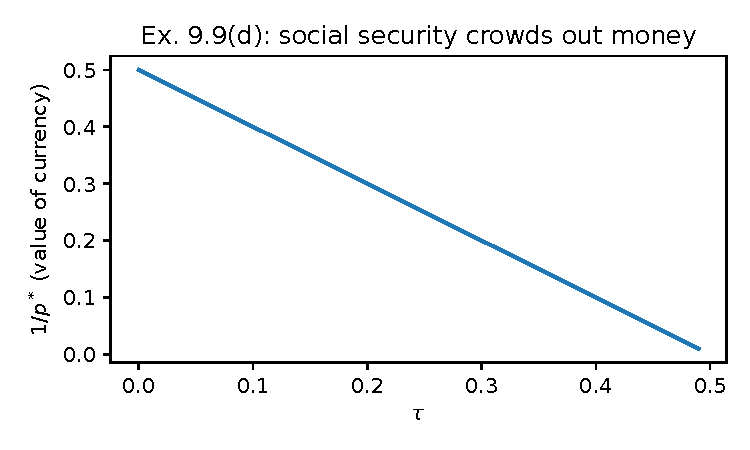
\includegraphics[width=0.6\linewidth]{fig/ls09_9_9_socsec.pdf}\\[3pt]
\captionof{figure}{Exercise 9.9(d). Value of currency in the stationary equilibrium against $\tau$
($y=N=H=1$).}
\end{center}

\begin{tcolorbox}[databox]
$y=N=H=1$, $\tau\in\{0,.1,.3,.45\}$: stationary $m=s(1)$ (closed form and numerical), and the
allocation is $(y/2,y/2)$. The closed-form continuum solves the recursion for $c\in\{0,.5\}$.
\end{tcolorbox}
\end{tcolorbox}

%------- 9.10 -------
\begin{tcolorbox}[evenbox,title={Exercise 9.10 \quad Seignorage}]
\begin{tcolorbox}[questionbox]
pp.~373--375. Consider an economy consisting of overlapping generations of two-period-lived agents.
At each date $t\ge1$, there are born $N_1$ ``lenders'' who are endowed with $\alpha>0$ units of the
single consumption good when they are young and zero units when they are old. At each date $t\ge1$,
there are also born $N_2$ ``borrowers'' who are endowed with zero units of the consumption good when
they are young and $\beta>0$ units when they are old. The good is nonstorable, and $N_1$ and $N_2$ are
constant through time. The economy starts at time 1, at which time there are $N$ old people who are
in the aggregate endowed with $H(0)$ units of unbacked, intrinsically worthless pieces of paper called
dollars. Assume that $\alpha,\beta,N_1$, and $N_2$ are such that
\[
\frac{N_2\beta}{N_1\alpha}<1.
\]
Assume that everyone has preferences
\[
u[c_t^h(t),c_t^h(t+1)]=\ln c_t^h(t)+\ln c_t^h(t+1),
\]
where $c_t^h(s)$ is consumption of time $s$ good of agent $h$ born at time $t$.

\textbf{a.} Compute the equilibrium interest rate on consumption loans in the equilibrium without
valued currency.

\textbf{b.} Construct a \emph{brief} argument to establish whether or not the equilibrium without
valued currency is Pareto optimal.

The economy also contains a government that purchases and destroys $G_t$ units of the good in period
$t$, $t\ge1$. The government finances its purchases entirely by currency creation. That is, at time
$t$,
\[
G_t=\frac{H(t)-H(t-1)}{p(t)},
\]
where $[H(t)-H(t-1)]$ is the additional dollars printed by the government at $t$ and $p(t)$ is the
price level at $t$. The government is assumed to increase $H(t)$ according to
\[
H(t)=zH(t-1),\qquad z\ge1,
\]
where $z$ is a constant for all time $t\ge1$.

At time $t$, old people who carried $H(t-1)$ dollars between $(t-1)$ and $t$ offer these $H(t-1)$
dollars in exchange for time $t$ goods. Also at $t$ the government offers $H(t)-H(t-1)$ dollars for
goods, so that $H(t)$ is the total supply of dollars at time $t$, to be carried over by the young into
time $(t+1)$.

\textbf{c.} Assume that $1/z>N_2\beta/N_1\alpha$. Show that under this assumption there exists a
continuum of equilibria with valued currency.

\textbf{d.} Display the unique stationary equilibrium with valued currency in the form of a
``quantity theory'' equation. Compute the equilibrium rate of return on currency and consumption
loans.

\textbf{e.} Argue that if $1/z<N_2\beta/N_1\alpha$, then there exists no valued-currency equilibrium.
Interpret this result. (\emph{Hint:} Look at the rate of return on consumption loans in the
equilibrium without valued currency.)

\textbf{f.} Find the value of $z$ that \emph{maximizes} the government's $G_t$ in a stationary
equilibrium. Compare this with the largest value of $z$ that is compatible with the existence of a
valued-currency equilibrium.
\end{tcolorbox}

\textbf{Solution:} Let $A\equiv N_1\alpha$ and $B\equiv N_2\beta z$. Aggregate saving at gross return
$R$ is $S(R)=\frac12(N_1\alpha-N_2\beta/R)$ (section 9.8).

\textbf{(a)} $S(R)=0$ gives $\boxed{1+r=N_2\beta/(N_1\alpha)<1}$.

\textbf{(b)} \textbf{Not optimal.} By Balasko--Shell (9.7.18), the constant interest factor
$\rho=N_2\beta/(N_1\alpha)<1$ gives $\sum_t\rho^t<\infty$. Directly, take $\varepsilon>0$ from each
young lender and hand it to the old lenders of the previous generation (to the initial old at $t=1$:
$N_1\varepsilon/N$ each). Borrowers keep their allocation. Feasibility holds at every date. A lender's
utility changes by
$\ln(\frac\alpha2-\varepsilon)+\ln(\frac{\rho\alpha}2+\varepsilon)-\ln\frac\alpha2-\ln\frac{\rho\alpha}2
\approx\varepsilon\big(\frac2{\rho\alpha}-\frac2\alpha\big)>0$ for small $\varepsilon$, since $\rho<1$.
The initial old gain too. This is a Pareto improvement.

\textbf{(c)} Let $m_t=H(t)/p(t)$ be aggregate real balances. The currency return is
$R_t=\frac{p(t)}{p(t+1)}=\frac{m_{t+1}}{m_t}\frac{H(t)}{H(t+1)}=\frac{m_{t+1}}{zm_t}$, and loans pay the
same. The young hold all currency: $S(R_t)=m_t$, that is $m_t=\frac12\big(A-\frac{N_2\beta zm_t}{m_{t+1}}\big)$.
Solve for $m_{t+1}$ and invert:
\[
m_{t+1}=\frac{Bm_t}{A-2m_t}\quad\Longrightarrow\quad x_{t+1}=\frac AB\,x_t-\frac2B,\qquad x_t\equiv\frac1{m_t}.
\]
This is linear, with fixed point $x^*=2/(A-B)$, positive iff $A>B$, which is $1/z>N_2\beta/(N_1\alpha)$.
Then $x_t-x^*=(A/B)^{t-1}(x_1-x^*)$ with $A/B>1$. Every $x_1\ge x^*$, that is $m_1\in(0,m^*]$ with
$m^*=(A-B)/2$, keeps $x_t>0$ and is an equilibrium. $x_1<x^*$ drives $x_t$ negative. This gives a
\textbf{continuum} indexed by $p(1)=zH(0)/m_1\ge zH(0)/m^*$, all but one with $m_t\to0$. (The
old's $H(0)$ plus the new issue $H(1)-H(0)$ make up $H(1)$; at $t=1$ the condition $S(R_1)=m_1$ holds
as written.)

\textbf{(d)} Stationary: $m_t=m^*=\frac12(N_1\alpha-N_2\beta z)$, so
\[
\boxed{p(t)=\frac{2}{N_1\alpha-N_2\beta z}\,H(t)},\qquad R=\frac1z\ \text{on currency and on loans},
\qquad G=\Big(1-\frac1z\Big)m^*.
\]
The price level grows at the money growth rate $z$.

\textbf{(e)} If $A<B$, then $x^*<0$ and $A/B<1$. The linear map sends every $x_1>0$ toward $x^*<0$,
so $x_t<0$ in finite time: $m_t$ explodes past $A/2$. If $A=B$, $x_{t+1}=x_t-2/B$, which also turns
negative. \textbf{No valued-currency equilibrium exists.} \emph{Interpretation.} In the long run
currency returns at most $1/z$. If $1/z$ is below the nonmonetary loan rate $N_2\beta/(N_1\alpha)$,
borrowers' demand at that rate exceeds lenders' supply ($S(1/z)<0$): nobody is left to hold money. The
inflation tax is too high relative to the private market's interest rate.

\textbf{(f)} $G(z)=\frac12\big(1-\frac1z\big)(N_1\alpha-N_2\beta z)
=\frac12\big[N_1\alpha+N_2\beta-N_2\beta z-\frac{N_1\alpha}z\big]$. So
$G'(z)=\frac12\big[-N_2\beta+\frac{N_1\alpha}{z^2}\big]=0$ and $G''<0$:
\[
\boxed{z^*=\sqrt{\frac{N_1\alpha}{N_2\beta}}},\qquad G(z^*)=\tfrac12\big(\sqrt{N_1\alpha}-\sqrt{N_2\beta}\big)^2 .
\]
The largest admissible $z$ is $\bar z=N_1\alpha/(N_2\beta)$ (the supremum; at $\bar z$, $G=0$). Since
$\bar z>1$, $z^*=\sqrt{\bar z}\in(1,\bar z)$. The revenue-maximising money growth rate is the square
root of the maximal one. Rates in $(z^*,\bar z)$ are on the wrong side of the Laffer curve.

\begin{center}
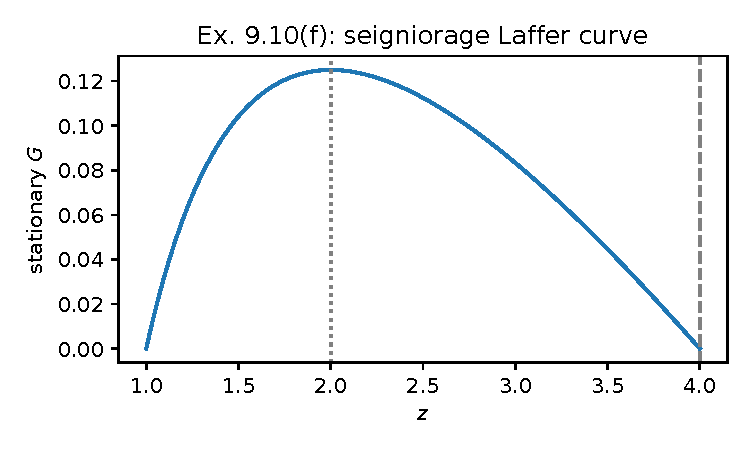
\includegraphics[width=0.6\linewidth]{fig/ls09_9_10_laffer.pdf}\\[3pt]
\captionof{figure}{Exercise 9.10(f). Stationary seigniorage $G(z)$ for $N_1=N_2=\alpha=1$,
$\beta=.25$. Dotted: $z^*=2$; dashed: $\bar z=4$.}
\end{center}

\begin{tcolorbox}[databox]
$N_1=N_2=\alpha=1$, $\beta=.25$, $z=2$: $m^*$ is a fixed point, $m_1=.5m^*$ gives $m_t\to0$,
$1/m_t$ satisfies the linear recursion exactly, and $m_1=1.01m^*$ explodes. With $z=1.2\bar z$, all
$m_1\in\{10^{-4},.01,.1,.3\}$ fail. A grid maximiser of $G$ gives $z^*=2$ and $G^*=.125$.
\end{tcolorbox}
\end{tcolorbox}

%------- 9.11 -------
\begin{tcolorbox}[oddbox,title={Exercise 9.11 \quad Unpleasant monetarist arithmetic}]
\begin{tcolorbox}[questionbox]
pp.~375--376. Consider an economy in which the aggregate demand for government currency for $t\ge1$
is given by $[M(t)p(t)]^d=g[R_1(t)]$, where $R_1(t)$ is the gross rate of return on currency between
$t$ and $(t+1)$, $M(t)$ is the stock of currency at $t$, and $p(t)$ is the value of currency in terms
of goods at $t$ (the reciprocal of the price level). The function $g(R)$ satisfies
\[
(1)\qquad g(R)(1-R)=h(R)>0\qquad\text{for }R\in(\underline R,1),
\]
where $h(R)\le0$ for $R<\underline R$, $R\ge1$, $\underline R>0$ and where $h'(R)<0$ for $R>R_m$,
$h'(R)>0$ for $R<R_m$, $h(R_m)>D$, where $D$ is a positive number to be defined shortly. The
government faces an infinitely elastic demand for its interest-bearing bonds at a
constant-over-time gross rate of return $R_2>1$. The government finances a budget deficit $D$,
defined as government purchases minus explicit taxes, that is constant over time. The government's
budget constraint is
\[
(2)\qquad D=p(t)[M(t)-M(t-1)]+B(t)-B(t-1)R_2,\qquad t\ge1,
\]
subject to $B(0)=0$, $M(0)>0$. In equilibrium,
\[
(3)\qquad M(t)p(t)=g[R_1(t)].
\]
The government is free to choose paths of $M(t)$ and $B(t)$, subject to equations (2) and (3).

\textbf{a.} Prove that, for $B(t)=0$, for all $t>0$, there exist two stationary equilibria for this
model.

\textbf{b.} Show that there exist values of $B>0$, such that there exist stationary equilibria with
$B(t)=B$, $M(t)p(t)=Mp$.

\textbf{c.} Prove a version of the following proposition: among stationary equilibria, the lower the
value of $B$, the lower the stationary rate of inflation consistent with equilibrium. (You will have
to make an assumption about Laffer curve effects to obtain such a proposition.)

This problem displays some of the ideas used by Sargent and Wallace (1981). They argue that, under
assumptions like those leading to the proposition stated in part c, the ``looser'' money is today
[that is, the higher $M(1)$ and the lower $B(1)$], the lower the stationary rate of inflation.
\end{tcolorbox}

\textbf{Solution:} Here $p(t)$ is the \emph{value} of currency, so $R_1(t)=p(t+1)/p(t)$, and gross
inflation is $1/R_1$. \emph{Reading.} The hypotheses on $h$ presume $h$ is continuous (it is
differentiable), and ``$h(R_m)>D$'' is a separate clause (a comma is missing in the statement).

\textbf{(a)} In a stationary equilibrium $R_1(t)=R$, so $M(t)p(t)=g(R)$ and
$p(t)M(t-1)=\frac{p(t)}{p(t-1)}\,p(t-1)M(t-1)=Rg(R)$. With $B\equiv0$, (2) becomes
\[
D=g(R)-Rg(R)=g(R)(1-R)=h(R).
\]
$h$ is continuous and $h(\underline R)\le0<D<h(R_m)$. By the intermediate value theorem there is a
root in $(\underline R,R_m)$, and it is unique there because $h'>0$. Likewise $h(1)\le0<D<h(R_m)$ gives
a unique root in $(R_m,1)$ because $h'<0$ there. So there are \textbf{exactly two} stationary
equilibria, $\underline R<R^{\rm bad}<R_m<R^{\rm good}<1$. At $t=1$, (2) reads
$D=g(R)-p(1)M(0)$, which gives $p(1)=Rg(R)/M(0)>0$. Then $M(t)=g(R)/[p(1)R^{t-1}]$ grows at $1/R$.

\textbf{(b)} With $B(t)=B$ for $t\ge1$, (2) for $t\ge2$ is $D=h(R)+B-R_2B$, that is
\[
h(R)=D+(R_2-1)B .
\]
The right side exceeds $D$ because $R_2>1$. By the argument of (a), two stationary roots exist
whenever $D+(R_2-1)B<h(R_m)$, i.e. for all
$\boxed{0<B<\bar B\equiv\dfrac{h(R_m)-D}{R_2-1}}$, which is a nonempty interval because $h(R_m)>D$.
At $B=\bar B$ the two roots merge at $R_m$. At $t=1$, $D=g(R)-p(1)M(0)+B$, so
$p(1)M(0)=g(R)+B-D$.

\textbf{(c)} Differentiate $h(R)=D+(R_2-1)B$: $h'(R)\,dR=(R_2-1)\,dB$, so
$\frac{dR}{dB}=\frac{R_2-1}{h'(R)}$. \emph{Assumption:} the economy is on the good side of the
Laffer curve, $R\in(R_m,1)$, where $h'<0$. This is the equilibrium selected by the adaptive and
learning dynamics discussed in section 9.5.1. Then $dR/dB<0$, and gross inflation $1/R$ rises with
$B$. \textbf{The lower $B$, the higher $R$ and the lower stationary inflation.} On the bad side
($h'>0$) the sign flips. Interpretation: selling bonds today ($B(1)$ up, $M(1)$ down, i.e.
``tighter'' money now) commits the government to interest payments $(R_2-1)B$ forever. These must
be covered by more seigniorage $h(R)$, which on the good side requires more inflation.

\begin{center}
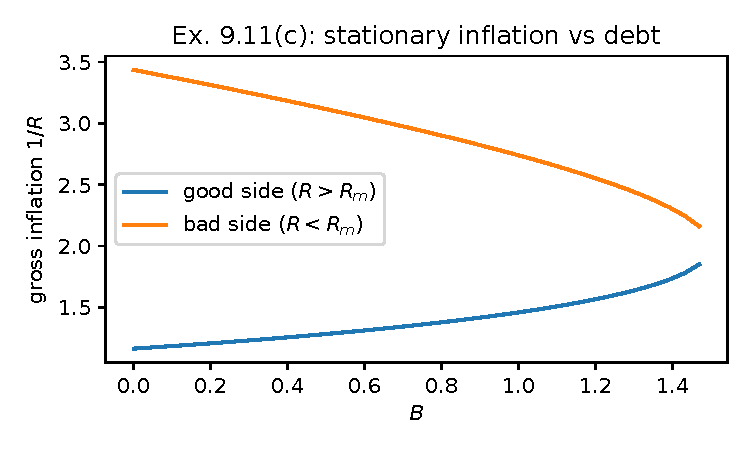
\includegraphics[width=0.6\linewidth]{fig/ls09_9_11_debt.pdf}\\[3pt]
\captionof{figure}{Exercise 9.11(c). Stationary gross inflation $1/R$ against $B$ on both sides of
the Laffer curve. Example: $g(R)=(1-.25/R)/2$, $D=.05$, $R_2=1.05$.}
\end{center}

\begin{tcolorbox}[databox]
Example demand (chosen): $g(R)=\frac12(w_1-w_2/R)$, the log-OLG saving function with $w_1=1$,
$w_2=.25$. Then $h$ has $\underline R=.25$, $R_m=.5$ (numerical maximiser), $h(R_m)=.125$; $D=.05$,
$R_2=1.05$, $\bar B=1.5$. For 40 values of $B\in[0,.98\bar B]$, \texttt{brentq} roots equal the
quadratic $w_1R^2-(w_1+w_2-2[D+(R_2-1)B])R+w_2=0$. $R^{\rm good}$ falls from $.8589$ to $.5403$
and $R^{\rm bad}$ rises. $p(1)M(0)>0$ throughout.
\end{tcolorbox}
\end{tcolorbox}

%------- 9.12 -------
\begin{tcolorbox}[evenbox,title={Exercise 9.12 \quad Grandmont--Hall}]
\begin{tcolorbox}[questionbox]
pp.~376--377. Consider a nonstochastic, one-good overlapping generations model consisting of
two-period-lived young people born in each $t\ge1$ and an initial group of old people at $t=1$ who
are endowed with $H(0)>0$ units of unbacked currency at the beginning of period 1. The one good in
the model is not storable. Let the aggregate first-period saving function of the young be
time-invariant and be denoted $f[1+r(t)]$ where $[1+r(t)]$ is the gross rate of return on
consumption loans between $t$ and $(t+1)$. The saving function is assumed to satisfy
$f(0)=-\infty$, $f'(1+r)>0$, $f(1)>0$.

Let the government pay interest on currency, starting in period 2 (to holders of currency between
periods 1 and 2). The government pays interest on currency at a nominal rate of
$[1+r(t)]p(t+1)/\bar p$, where $[1+r(t)]$ is the real gross rate of return on consumption loans,
$p(t)$ is the price level at $t$, and $\bar p$ is a target price level chosen to satisfy
\[
\bar p=H(0)/f(1).
\]
The government finances its interest payments by printing new money, so that the government's budget
constraint is
\[
H(t+1)-H(t)=\Big\{[1+r(t)]\frac{p(t+1)}{\bar p}-1\Big\}H(t),\qquad t\ge1,
\]
given $H(1)=H(0)>0$. The gross rate of return on consumption loans in this economy is $1+r(t)$. In
equilibrium, $[1+r(t)]$ must be at least as great as the real rate of return on currency
\[
1+r(t)\ge[1+r(t)]p(t)/\bar p=[1+r(t)]\frac{p(t+1)}{\bar p}\frac{p(t)}{p(t+1)}
\]
with equality if currency is valued,
\[
1+r(t)=[1+r(t)]p(t)/\bar p,\qquad 0<p(t)<\infty.
\]
The loan market-clearing condition in this economy is
\[
f[1+r(t)]=H(t)/p(t).
\]

\textbf{a.} Define an equilibrium.

\textbf{b.} Prove that there exists a unique monetary equilibrium in this economy and compute it.
\end{tcolorbox}

\textbf{Solution:}

\textbf{(a)} An \emph{equilibrium} is a sequence $\{1+r(t),p(t),H(t)\}_{t\ge1}$ with $H(1)=H(0)$ that
satisfies four conditions. (i) The budget constraint
$H(t+1)=[1+r(t)]\frac{p(t+1)}{\bar p}H(t)$. (ii) The arbitrage condition
$1+r(t)\ge[1+r(t)]p(t)/\bar p$, with equality when currency is valued. (iii) Loan-market clearing
$f[1+r(t)]=H(t)/p(t)$. (iv) The young's saving is optimal, which is embodied in $f$. It is
\emph{monetary} if $0<p(t)<\infty$ for all $t$.

\textbf{(b)} \emph{Price level.} In a monetary equilibrium the arbitrage condition holds with
equality: $1+r(t)=[1+r(t)]p(t)/\bar p$. Since $1+r(t)>0$, this gives $\boxed{p(t)=\bar p}$ for all $t$.
\emph{Interest rate.} At $t=1$, clearing gives $f[1+r(1)]=H(1)/\bar p=H(0)/\bar p=f(1)$. Since $f$ is
strictly increasing, $1+r(1)=1$. \emph{Induction.} Suppose $1+r(t)=1$ and $H(t)=H(0)$. Then (i) gives
$H(t+1)=1\cdot\frac{\bar p}{\bar p}H(t)=H(0)$, and clearing at $t+1$ gives $f[1+r(t+1)]=f(1)$, so
$1+r(t+1)=1$. Hence
\[
\boxed{p(t)=\bar p=\frac{H(0)}{f(1)},\qquad 1+r(t)=1,\qquad H(t)=H(0)\qquad\forall t\ge1}
\]
is the unique monetary equilibrium. It exists because $f(1)>0$ makes $\bar p$ positive and finite.
\emph{Why uniqueness.} Paying interest indexed to the price gap removes the continuum of 9.1(e).
Any $p(t)\ne\bar p$ would give currency a real return different from loans. Given $p=\bar p$, the
system $f[1+r(t+1)]=[1+r(t)]f[1+r(t)]$ is \emph{unstable} at $1+r=1$ (slope $1+f(1)/f'(1)>1$). Paths
starting at $1+r(1)\ne1$ either explode or drift to autarky, and the initial condition $H(1)=H(0)$
rules them all out. The condition $f(0)=-\infty$ guarantees that the nonmonetary loan market has a
positive clearing rate. It is not needed for the monetary equilibrium.

\begin{tcolorbox}[databox]
$f(R)=\frac12(1-.5/R)$ (so $f(1)=.25$), $H(0)=1$: $\bar p=4$. \texttt{brentq} gives $1+r(1)=1$, and
the recursion maps $1$ to $1$. Starting at $1\pm10^{-6}$, the deviation doubles per period (slope
$1+f(1)/f'(1)=2$). The upper path becomes infeasible in finite time. The lower one converges to the
autarkic $w_2/w_1=.5$ but violates $f[1+r(1)]=H(0)/\bar p$.
\end{tcolorbox}
\end{tcolorbox}

%------- 9.13 -------
\begin{tcolorbox}[oddbox,title={Exercise 9.13 \quad Bryant--Keynes--Wallace}]
\begin{tcolorbox}[questionbox]
pp.~377--378. Consider an economy consisting of overlapping generations of two-period-lived agents.
There is a constant population of $N$ young agents born at each date $t\ge1$. There is a single
consumption good that is not storable. Each agent born in $t\ge1$ is endowed with $w_1$ units of the
consumption good when young and with $w_2$ units when old, where $0<w_2<w_1$. Each agent born at
$t\ge1$ has identical preferences $\ln c_t^h(t)+\ln c_t^h(t+1)$, where $c_t^h(s)$ is time $s$
consumption of agent $h$ born at time $t$. In addition, at time 1, there are alive $N$ old people who
are endowed with $H(0)$ units of unbacked paper currency and who want to maximize their consumption
of the time 1 good.

A government attempts to finance a constant level of government purchases $G(t)=G>0$ for $t\ge1$ by
printing new base money. The government's budget constraint is
\[
G=[H(t)-H(t-1)]/p(t),
\]
where $p(t)$ is the price level at $t$, and $H(t)$ is the stock of currency carried over from $t$ to
$(t+1)$ by agents born in $t$. Let $g=G/N$ be government purchases per young person. Assume that
purchases $G(t)$ yield no utility to private agents.

\textbf{a.} Define a stationary equilibrium with valued fiat currency.

\textbf{b.} Prove that, for $g$ sufficiently small, there exists a stationary equilibrium with valued
fiat currency.

\textbf{c.} Prove that, in general, if there exists one stationary equilibrium with valued fiat
currency, with rate of return on currency $1+r(t)=1+r_1$, then there exists at least one other
stationary equilibrium with valued currency with $1+r(t)=1+r_2\ne1+r_1$.

\textbf{d.} Tell whether the equilibria described in parts b and c are Pareto optimal, among
allocations among private agents of what is left after the government takes $G(t)=G$ each period.
(A proof is not required here: an informal argument will suffice.)

Now let the government institute a forced saving program of the following form. At time 1, the
government redeems the outstanding stock of currency $H(0)$, exchanging it for government bonds. For
$t\ge1$, the government offers each young consumer the option of saving at least $F$ worth of time
$t$ goods in the form of bonds bearing a constant rate of return $(1+r_2)$. A legal prohibition
against private intermediation is instituted that prevents two or more private agents from sharing
one of these bonds. The government's budget constraint for $t\ge2$ is
\[
G/N=B(t)-B(t-1)(1+r_2),
\]
where $B(t)\ge F$. Here $B(t)$ is the saving of a young agent at $t$. At time $t=1$, the government's
budget constraint is
\[
G/N=B(1)-\frac{H(0)}{Np(1)},
\]
where $p(1)$ is the price level at which the initial currency stock is redeemed at $t=1$. The
government sets $F$ and $r_2$.

Consider stationary equilibria with $B(t)=B$ for $t\ge1$ and $r_2$ and $F$ constant.

\textbf{e.} Prove that if $g$ is small enough for an equilibrium of the type described in part a to
exist, then a stationary equilibrium with forced saving exists. (Either a graphical argument or an
algebraic argument is sufficient.)

\textbf{f.} Given $g$, find the values of $F$ and $r_2$ that maximize the utility of a
representative young agent for $t\ge1$.

\textbf{g.} Is the equilibrium allocation associated with the values of $F$ and $(1+r_2)$ found in
part f optimal among those allocations that give $G(t)=G$ to the government for all $t\ge1$? (Here an
informal argument will suffice.)
\end{tcolorbox}

\textbf{Solution:} Let $R=1+r$ be the return on currency, $s(R)=\frac12(w_1-w_2/R)$ from (T1), and
$m_t=H(t)/(Np(t))$.

\textbf{(a)} A \emph{stationary equilibrium with valued currency} is a constant $R\in(0,\infty)$ and
constant real balances $m>0$ per young person, with $p(t)=p(1)R^{1-t}$ and $H(t)=Nmp(t)$, such that
three conditions hold. (i) The young optimise: $m=s(R)$. (ii) The budget holds:
$g=\frac{H(t)-H(t-1)}{Np(t)}=m-m\frac{p(t-1)}{p(t)}=m(1-R)$ for $t\ge2$. (iii) At $t=1$,
$Nm=H(0)/p(1)+G$, which fixes $p(1)$. Combining (i) and (ii):
\[
g=s(R)(1-R)\equiv h(R)=\tfrac12\Big(w_1-\frac{w_2}R\Big)(1-R),
\]
which is (9.5.5a) with $d=g$.

\textbf{(b)} $h$ is continuous on $[w_2/w_1,1]$, zero at both ends and positive inside.
$h'(R)=\frac12\big(-w_1+\frac{w_2}{R^2}\big)=0$ at $R_m=\sqrt{w_2/w_1}$, where
$h_{\max}=\frac12(\sqrt{w_1}-\sqrt{w_2})^2$. For $0<g\le h_{\max}$, a root $R\in(w_2/w_1,1)$ exists by
the intermediate value theorem. It has $s(R)>0$ and gives $p(1)=H(0)/(N[s(R)-g])=H(0)/(NRs(R))>0$.
So for $g$ small enough ($g\le h_{\max}$) a stationary monetary equilibrium exists.

\textbf{(c)} Multiply $h(R)=g$ by $2R$: $w_1R-w_1R^2-w_2+w_2R=2gR$, that is
\[
w_1R^2-(w_1+w_2-2g)R+w_2=0,\qquad R_1R_2=\frac{w_2}{w_1}.
\]
If $R_1=1+r_1$ is a root, then $R_2=w_2/(w_1R_1)$ is the other one. It lies in $(w_2/w_1,1)$ because
$R_1$ does, and it is also an equilibrium. $R_2\ne R_1$ unless $R_1=\sqrt{w_2/w_1}$, i.e. unless
$g=h_{\max}$ exactly, the tangency case. That is why the statement says ``in general''.

\textbf{(d)} \textbf{Neither is Pareto optimal.} Stationary feasibility after $G$ is
$c_y+c_o=w_1+w_2-g$. The golden-rule allocation $c_y=c_o=\bar c\equiv(w_1+w_2-g)/2$, with $\bar c$
also given to the initial old, gives every generation the maximal stationary utility $2\ln\bar c$.
The equilibria have MRS $=R<1$, so they are off that point: $v(R)<2\ln\bar c$. The initial old get
$w_2+s(R)-g$, and $\bar c-[w_2+s(R)-g]=\frac12\big[\frac{w_2(1-R)}R+g\big]>0$. So the golden rule
Pareto dominates both. (Balasko--Shell: $\sum R^t<\infty$.) Between the two, the high-return
equilibrium $R_{\rm hi}>R_m$ Pareto dominates the low-return one. By (T2), savers' $v$ rises with $R$,
and the initial old's $w_2+s(R)-g$ rises with $R$.

\textbf{(e)} Take either stationary monetary equilibrium $\bar R$ from (b) and set
$\boxed{F=s(\bar R),\ 1+r_2=\bar R}$. At return $\bar R$, the young's unconstrained optimum is exactly
$s(\bar R)=F$, so they buy $B=F$ (which satisfies $B\ge F$). The budget for $t\ge2$ is
$B-B(1+r_2)=s(\bar R)(1-\bar R)=h(\bar R)=g$. At $t=1$, $p(1)=H(0)/(N[B-g])$, and $B-g=\bar
Rs(\bar R)>0$. So a stationary forced-saving equilibrium exists and replicates the monetary
allocation. Graphically, it is the same point as in Figure 9.2.4, with bonds in place of currency.

\textbf{(f)} Stationarity gives $g=B-B(1+r_2)$, so $(1+r_2)B=B-g$. The agent consumes
$c_y=w_1-B$ and $c_o=w_2+(1+r_2)B=w_2+B-g$. The government can implement any $B$ by setting $F=B$ and
$1+r_2=1-g/B$. Maximise $\ln(w_1-B)+\ln(w_2+B-g)$: the first-order condition
$\frac1{w_1-B}=\frac1{w_2+B-g}$ gives
\[
\boxed{F=B^*=\frac{w_1-w_2+g}2,\qquad 1+r_2=1-\frac g{B^*}=\frac{w_1-w_2-g}{w_1-w_2+g}},\qquad c_y=c_o=\bar c .
\]
\emph{Implementability.} At $1+r_2<1$ the agent's desired saving $s(1+r_2)$ is below $F$. The minimum
binds and the agent buys exactly $F$, provided this beats not buying at all:
$2\ln\bar c\ge\ln w_1+\ln w_2$. That holds iff $g\le(\sqrt{w_1}-\sqrt{w_2})^2=2h_{\max}$, which is
implied by $g\le h_{\max}$. The indivisibility of bonds, plus the ban on sharing them, is what stops
agents from undoing the minimum. That is the role of the legal restriction.

\textbf{(g)} \textbf{Yes.} The allocation gives $\bar c$ to both ages, and the initial old get
$w_2+B^*-g=\bar c$ as well. Its MRS equals $1=n$: an interest factor of 1 makes
$\sum_t\prod_s(1+r_s)=\infty$, so it is optimal by Balasko--Shell (constant population). Informally,
any reallocation that helps one generation must take from the next. The chain argument of section 9.7
($\theta=n$) shows the deficit then grows without bound, which is infeasible. This is the stationary
counterpart of 9.4--9.5, where the optimal equilibrium has return $n$. Forced saving at a negative
real rate collects $g$ as a lump sum on savers without distorting the margin, unlike the inflation
tax.

\begin{tcolorbox}[databox]
$w_1=1$, $w_2=.25$, $g=.05$: $R_{\rm lo}=.29105$ and $R_{\rm hi}=.85895$, with product $.25$. The high
root dominates for every generation and the initial old. The golden rule $\bar c=.6$ dominates both.
$F=s(\bar R)$, $1+r_2=\bar R$ satisfy the budget. A numerical maximiser gives $B^*=.4=F$ and
$1+r_2=.875$. At $.875$ the unconstrained saving is below $F$, and $2\ln\bar c>\ln w_1+\ln w_2$.
\end{tcolorbox}
\end{tcolorbox}

%======================================================================
\section*{Companion code}
\addcontentsline{toc}{section}{Companion code}
%======================================================================

Every numerical result above is reproduced by the notebook \texttt{ls\_ch09.ipynb} in this folder
(executed, outputs saved). Each claim is checked by an independent route with an \texttt{assert}.

\begin{center}
\begin{tabular}{@{}lp{11.6cm}@{}}
\toprule
\textbf{Section} & \textbf{What it checks} \\
\midrule
9.1 & CRRA saving closed form vs numerical optimisation; $s(1)=(w_1-w_2)/2$; forward map $m_t\to0$, $R_t\to(w_2/w_1)^\gamma$; figure. \\
9.2 & Loan-market root; price-path closed form vs recursion; money-market clearing; lenders vs borrowers welfare. \\
9.3 & Quadratic vs \texttt{brentq} tree price ($\gamma=1,2$); instability of $a_1\ne\bar a$; unbounded tree value. \\
9.4--9.5 & $R=n$; closed-form $p_t$ vs recursion; limits of $R_t$; Pareto ranking in $c$; nonexistence for $nw_1\le w_2$. \\
9.6 & Kareken--Wallace continuum in $e$; constant-split $e$; nominal-anchor prices in (d). \\
9.7--9.8 & Loan-market roots; $x\mapsto x/(1-x)$ exit; $q=8/y$; feasibility; welfare; inside-money clearing. \\
9.9--9.10 & Social-security continuum and crowding out (figure); linear $1/m$ dynamics; Laffer maximum (figure). \\
9.11 & Two stationary roots vs quadratic; comparative statics in $B$ (figure). \\
9.12 & $p=\bar p$, $1+r=1$; instability of the recursion. \\
9.13 & Root product; Pareto comparisons; forced-saving replication and optimum. \\
\bottomrule
\end{tabular}
\end{center}

Figures are saved to \texttt{fig/ls09\_*.pdf} with TrueType (not Type~3) fonts.

\end{document}
